\documentclass{article}
\usepackage[left=2cm, right=2cm, top=2cm, bottom=3cm]{geometry}
\usepackage{amsmath} % provides many mathematical environments & tools

\setlength{\parindent}{0mm}

\usepackage{graphicx}
\graphicspath{ {./images/} }

\begin{document}

\title{Real Number Theory Analysis of Special Functions Through Divisor Waves and Extreme Operators}
\author{Leo J. Borcherding}
\date{\today}
\maketitle

\subsection*{DIVISOR WAVES}
DIVISOR WAVES - This paper bases most of its findings on representative trigonometric functions called Divisor Waves. Throughout the paper, these Wave functions will only be written using sine waves. However, they could also be changed and written with cosine.
Divisor Waves, or DW, act as a means of checking whether a given number is divisible by the number associated with the DW. For example, the DW for 2, also called DW-2 and found below as equation (1), is a sine wave that has x-intercepts at all multiples of 2. This means that all numbers which are divisible by 2 are the zeros of DW-2, hence the Divisor in Divisor Wave.

\begin{align*}
	f(z) = |2\sin\left(\frac{\pi z}{2}\right)|
\end{align*} 

Looking further at equation (1) you will see there is a pi coefficient inside of the sine function, this is there to ensure that the wave does not have a period of radians but rather, ordinary numbers. For scaling purposes that aren’t required, a 2 is also added in front to ensure that the amplitude of each DW is that of its associated whole number. 

\begin{align*}
  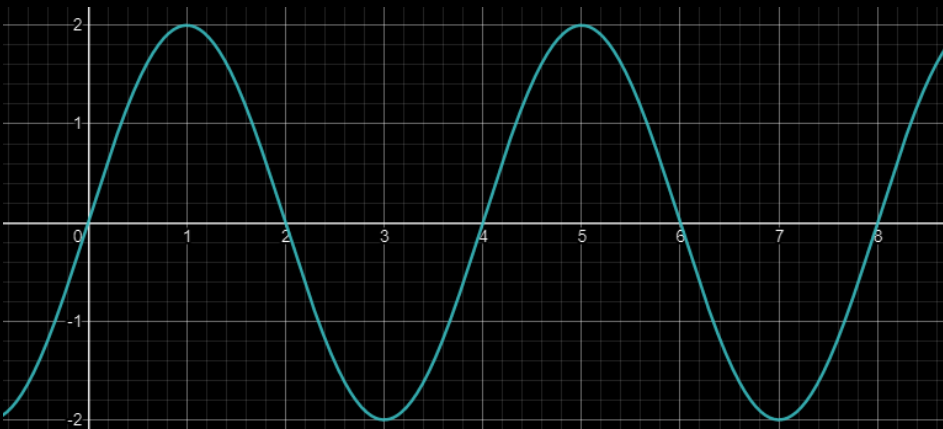
\includegraphics[scale=0.4]{graphs/2D_Real_Graphs/DW_2}
\end{align*}

Iterating this process, we will create a DW for each whole number like so: 

\begin{align*}
	f2(z) = |2\sin\left(\frac{\pi z}{2}\right)| \\
	f3(z) = |3\sin\left(\frac{\pi z}{3}\right)| \\
	f4(z) = |4\sin\left(\frac{\pi z}{4}\right)|	\\
	f5(z) = |5\sin\left(\frac{\pi z}{5}\right)| \\
	f6(z) = |6\sin\left(\frac{\pi z}{6}\right)|	\\	
	...
\end{align*} 

Now that we have created a DW for every whole number, except for 1, we can look at many DWs on a graph where we can see the factors of each number.

Graph of the Sieve of Eratosthenes:

\begin{align*}
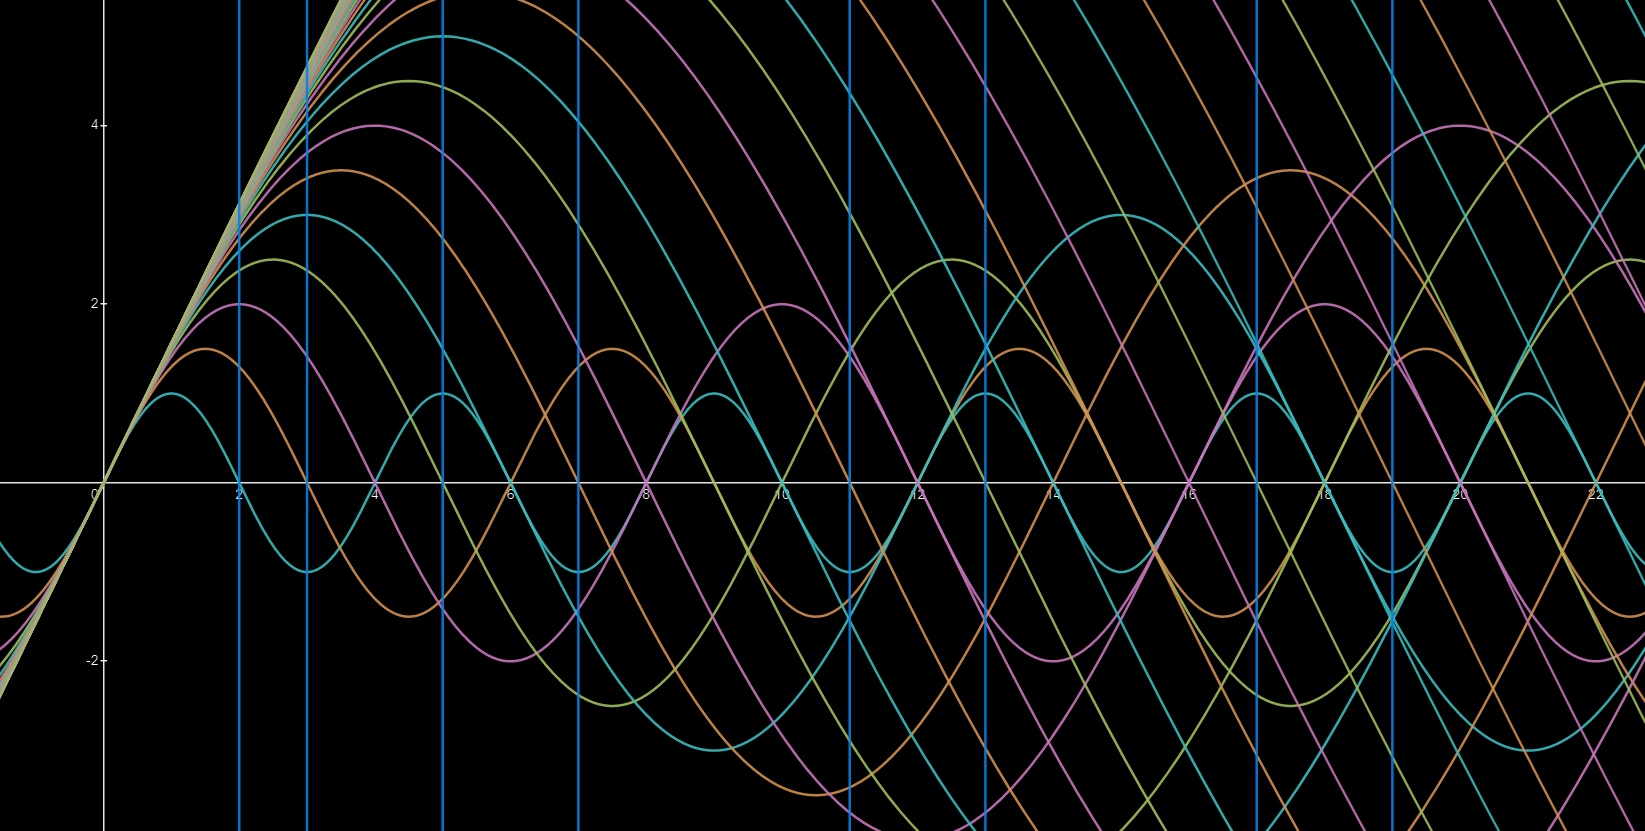
\includegraphics[scale=0.4]{graphs/2D_Real_Graphs/sieve_2}
\end{align*}

By doing this, we have essentially created the Sieve of Eratosthenes using sine waves. You will notice that at each prime number there is only 1 wave passing through it. If we had created a    DW-1 then there would be 2 waves passing through each prime. “A prime is only divisible by itself, and one.” Because we reject DW-1 and go straight to DW-2, this means the wave passing through any prime x-intercept is the DW-P where P is that prime number. I.e., DW-2, DW-3, DW-5, DW-7, DW-11, DW-13, etc. \\ 
\newline
Now that we have created an infinite number of waves, each representing a different factor, we can combine them into one wave function which has attributes from each wave. We do this by using an Infinite Product to define our set of infinitely many waves. Refer to the function a(z) in the next section.

\subsection*{Initial Description of Function a(z)}
In this paper, we will analyze several special functions using divisor waves and extreme operators. Specifically, we will consider the functions $A(z)$, $B(z)$, $C(z)$, $D(z)$, $E(z)$, $F(z)$, and the Riemann zeta function $\zeta(z)$.

We define the function $a(z)$ as follows:

\begin{align*}
	a(z) = |\prod_{n=2}^z \alpha\frac{z}{n}\sin\left(\frac{\pi z}{n}\right)|
\end{align*} 
	
The Function a(z) is the infinite product of sin(pi*z/n) where 2 is less than or equal to n is less than or equal to z. It is this function that provides a map of the prime, and composite numbers. The front term alpha*x/n is used for scaling purposes, as this function is highly explosive in the y-direction as you move down the x-axis. The alpha is just a coefficient that has a slider ranging from 0<alpha<2 and is used to stretch the function as needed. \\
\newline
The “abs” value in front ensures that this function stays above the x-axis. This has the same effect as y=abs[sin(x)]. On the inside of the sine function, we still have the pi coefficient but have now replaced the whole number associated with the DW with n so that we can test through an infinite number of whole numbers. \\

\begin{align*}
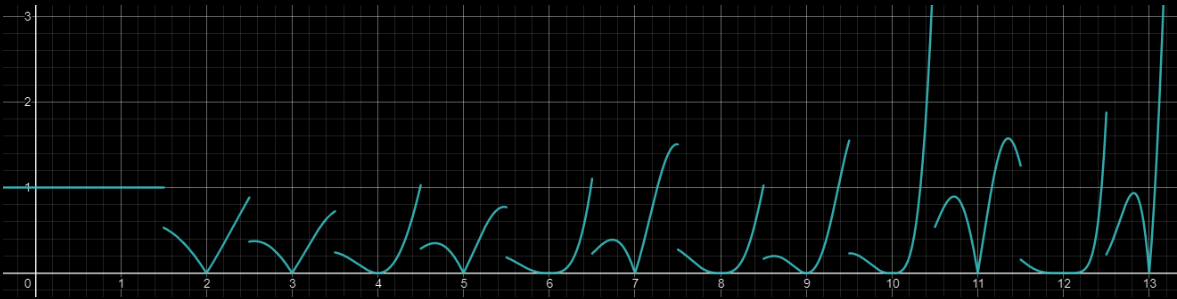
\includegraphics[scale=0.5]{graphs/2D_Real_Graphs/cuspcurve}
\end{align*}

The Function a(z) is the infinite product of sinusoidal Divisor Waves, this essentially combines them all into one resultant wave. Looking at the graph, you can see that at each prime number there is a cusp, and at each composite number there is a curve. This is because of the way the function approaches zero at that point. This Concept will apply to the proceeding functions as well and will allow us to analyze the continuity at each point and extract meaningful information. \\
\newline
COMPOSITE - At each composite number there are many waves all being combined at one point. For highly composite numbers there are more DWs that have x-intercepts causing them to start going to zero sooner. It is because of this that a curve is created. This is also true for normal composite numbers, but it happens slower than that of highly composite numbers. See 12 for an example of highly composite. \\
\newline
PRIME - Prime numbers do not approach zero the same way. For a prime number, there are also many waves combining at one point, but only DW-P has an x-intercept. This means that they only reach zero for a moment before returning to larger values, and this creates the cusp. \\

\subsection*{Initial Description of Function A(z)}
We define the Normalized a(z), function $A(z)$ as follows:
	
\begin{align*}
	A(z) = \frac{|\prod_{n=2}^z \alpha\frac{z}{n}\sin\left(\frac{\pi z}{n}\right)|^{-m}}{|\prod_{n=2}^z \alpha\frac{z}{n}\sin\left(\frac{\pi z}{n}\right)|^{-m}!}
\end{align*} 

\begin{align*}
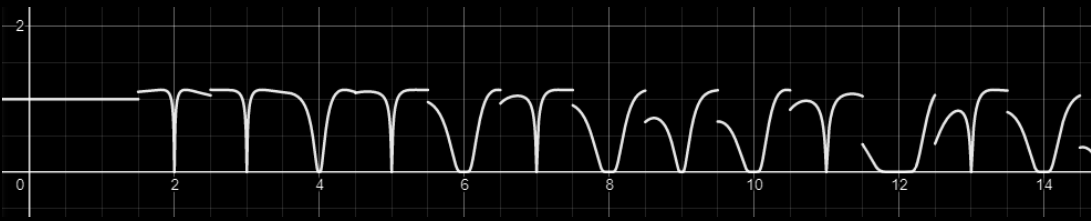
\includegraphics[scale=0.55]{graphs/2D_Real_Graphs/norm_cuspcurve}
\end{align*}

This process is similar to linearization. By taking the original function a(z) and taking the fraction:

\begin{align*}
a(z)^{-m}/(a(z)^{-m})!
\end{align*} 

We are utilizing the factorial function to remove the explosive nature of a(z) and the exponent -m is a coefficient on a slider. This coefficient will allow us to magnify the function similar to \alpha.

\subsection*{Initial Description of Function b(z)}
The function $b(z)$ is defined as the infinite product of the infinite product representation of $\sin(\pi*z/n)$:

\begin{align*}
	b(z) = |\prod_{n=2}^z \left[\frac{\beta z}{n}\left({\pi z}\prod_{k=2}^z\left(1 - \frac{z^2}{n^2k^2}\right)\right)\right]|
\end{align*}

\begin{align*}
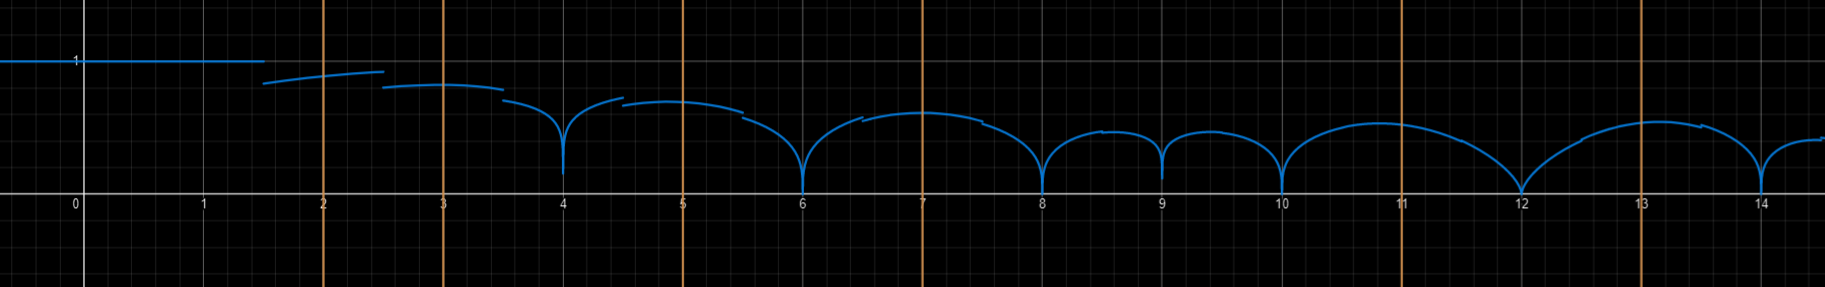
\includegraphics[scale=0.35]{graphs/2D_Real_Graphs/prime_indicator_og}
\end{align*}

Derivation of b(z) by substituting the infinite product representation of $sin(\pi*z/n)$ into the infinite product of $\sin(\pi*z/n)$: \\

Starting with function a(z): \\
\begin{align*}
	a(z) = |\prod_{n=2}^z \alpha\frac{z}{n}\sin\left(\frac{\pi z}{n}\right)| \\
\end{align*}

We use the Weierstrass Product Formula for sin to form the relationship where k is a constant: \\
\begin{align*}
	\sin\left(\frac{\pi z}{k}\right) = \pi z\prod_{n=2}^z \left(1-\frac{z^2}{n^2k^2}\right) \\
\end{align*}

Taking the product of both sides we have the functional equation of a(z) known as b(z): \\
\begin{align*}
	\prod_{k=2}^z\sin\left(\frac{\pi z}{k}\right) = \prod_{k=2}^z \pi z\prod_{n=2}^z \left(1-\frac{z^2}{n^2k^2}\right) \\
\end{align*}

Next, we substitute the formula for sin into the expression for $a(z)$, using $k=n$:
\begin{align*}
a(z) &= \left|\prod_{n=2}^z \alpha\frac{z}{n}\sin\left(\frac{\pi z}{n}\right)\right| \\
&= \left|\prod_{n=2}^z \alpha\frac{z}{n} \pi z\prod_{k=2}^n \left(1-\frac{z^2}{k^2n^2}\right)\right| \\
&= \left|\alpha^{z-1}\pi^z z^z \prod_{n=2}^z\prod_{k=2}^n \left(1-\frac{z^2}{k^2n^2}\right)\right| \\
&= \left|\alpha^{z-1}\pi^z z^z \prod_{k=2}^z\prod_{n=k}^z \left(1-\frac{z^2}{k^2n^2}\right)\right| \\
&= \left|\alpha^{z-1}\pi^z z^z \prod_{k=2}^z\prod_{n=1}^{z-k} \left(1-\frac{z^2}{k^2(k+n)^2}\right)\right| \\
\end{align*}

where in the last step we changed the order of the product by substituting $n\rightarrow n-k$. The resulting expression is known as the Barnes G-function and is denoted as $G(z+1)$. Therefore we have:
\begin{align*}
a(z) &= \left|\alpha^{z-1}\pi^z z^z G(z+1)\right| \\
\end{align*}

This proof shows the relationship between a(z) and b(z), and allows us to appreciate some of the beautiful relationships between these functions. The function b(z) is an equivalent form of a(z) however it has extra parameters that we can use to our advantage.

Now, we can expand the product out to infinity, using the expression we derived earlier:

\begin{align*}
f(x) &= \prod_{n=2}^{x} \left|\frac{\pi x}{n} \prod_{k=2}^{\infty} \left( 1 - \frac{x^2}{k^2 n^2} \right) \right| \\
&= \prod_{n=2}^{x} \left|\frac{\pi x}{n} \prod_{k=2}^{\infty} \left( 1 - \frac{x^2}{k^2 n^2} \right) \right| \\
&= \prod_{n=2}^{x} \pi x/n \left[ \left( 1 - \frac{x^2}{(2^2)(n^2)}\right) \left( 1 - \frac{x^2}{(3^2)(n^2)}\right) \left( 1 - \frac{x^2}{(4^2)(n^2)}\right) \cdots \right] \\
\end{align*}

\begin{align*}
&= \frac{\pi*x}{n}\left[ \left( 1 - \frac{x^2}{(2^2)(2^2)}\right) \left( 1 - \frac{x^2}{(2^2)(3^2)}\right) \left( 1 - \frac{x^2}{(2^2)(4^2)}\right) \cdots \right] \\
&\qquad \times \left[ \left( 1 - \frac{x^2}{(3^2)(2^2)}\right) \left( 1 - \frac{x^2}{(3^2)(3^2)}\right) \left( 1 - \frac{x^2}{(3^2)(4^2)}\right) \cdots \right] \\
&\qquad \times \left[ \left( 1 - \frac{x^2}{(4^2)(2^2)}\right) \left( 1 - \frac{x^2}{(4^2)(3^2)}\right) \left( 1 - \frac{x^2}{(4^2)(4^2)}\right) \cdots \right] \\
&\qquad \times \cdots \\
\end{align*}

We can now use this infinite polynomial to evaluate $x = 4$ and we can see that for the factors of 4 the terms go to zero. \\

\begin{flushleft*}
f(4) = \\
\end{flushleft*}

\begin{align*}
= \frac{\pi*x}{n}\left\left[ \left( 1 - \frac{4^2}{(2^2)(2^2)}\right) \left( 1 - \frac{4^2}{(2^2)(3^2)}\right) \left( 1 - \frac{4^2}{(2^2)(4^2)}\right) \cdots \right] \\
\times \left[ \left( 1 - \frac{4^2}{(3^2)(2^2)}\right) \left( 1 - \frac{4^2}{(3^2)(3^2)}\right) \left( 1 - \frac{4^2}{(3^2)(4^2)}\right) \cdots \right] \\
\times \left[ \left( 1 - \frac{4^2}{(4^2)(2^2)}\right) \left( 1 - \frac{4^2}{(4^2)(3^2)}\right) \left( 1 - \frac{4^2}{(4^2)(4^2)}\right) \cdots \right] \\
\times \cdots \\
= \cdots \left( 1 - \frac{4^2}{(2^2)(2^2)}\right) \cdots \\
= \left( 1 - \frac{4^2}{(4)(4)}\right) = 0 \\
\end{align*}

We can now take $b(z)$ and create the function $b(x+iy)$ where $z = x + iy$.
\begin{align*}
b(x+iy) = \left|\prod_{n=2}^{x+iy} \left[\frac{\beta (x+iy)}{n}\left({\pi (x+iy)}\prod_{k=2}^{x+iy}\left(1 - \frac{(x+iy)^2}{n^2k^2}\right)\right)\right]\right|
\end{align*}

2D Graph of $b(x+iy)$ showcasing the zeros of the composite numbers:
\begin{align*}
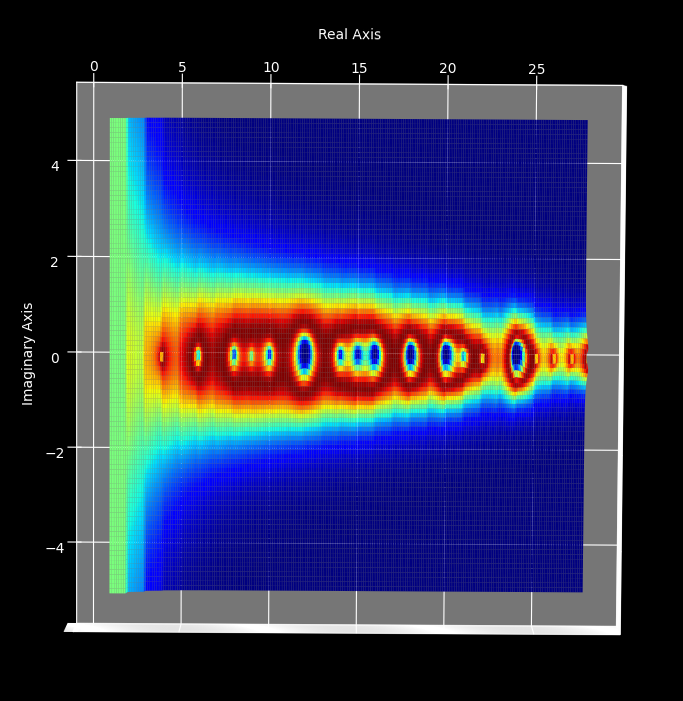
\includegraphics[scale=0.4]{graphs/3D_Complex_Graphs/product_of_product_representation_of_sin/ComplexPlot_prodprodforsin_1}
\end{align*}

The above plot, and following plots, were designed using matplotlib and python. The software designed for this paper is called Special Functions and it provides a way to graph these infinite products in the 3D complex plane using a heatmap colorization and height. We can see the zeros of $b(x + iy)$ as the blue troughs in the hills. These are the composite numbers. For each composite number there is a factor causing the product to go to zero. For all whole number values of x where x is prime, the function does not go to zero. We can observe this phenomenon at 11, and 13 on the graph as these are prime numbers. \\

3D Graph of $b(x+iy)$ showcasing the zeros of the composite numbers:
\begin{align*}
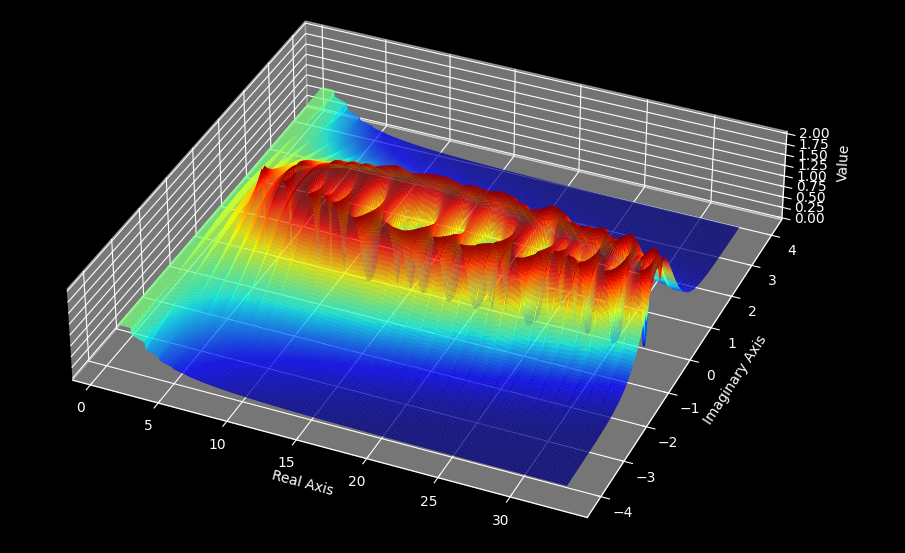
\includegraphics[scale=0.4]{graphs/3D_Complex_Graphs/product_of_product_representation_of_sin/ComplexPlot_prodprodforsin_9}
\end{align*}

The above graph is the 3D plot for $b(x+iy)$ where the 3rd dimension is height. This graph shows the complexity of the primes as it is solely dependant on the distribution of composite numbers. \\

2D Fractal $#1$ Graph of $b(x+iy)$ showcasing the zeros of the composite numbers by Multipling $b(x+iy) * iy$:
\begin{align*}
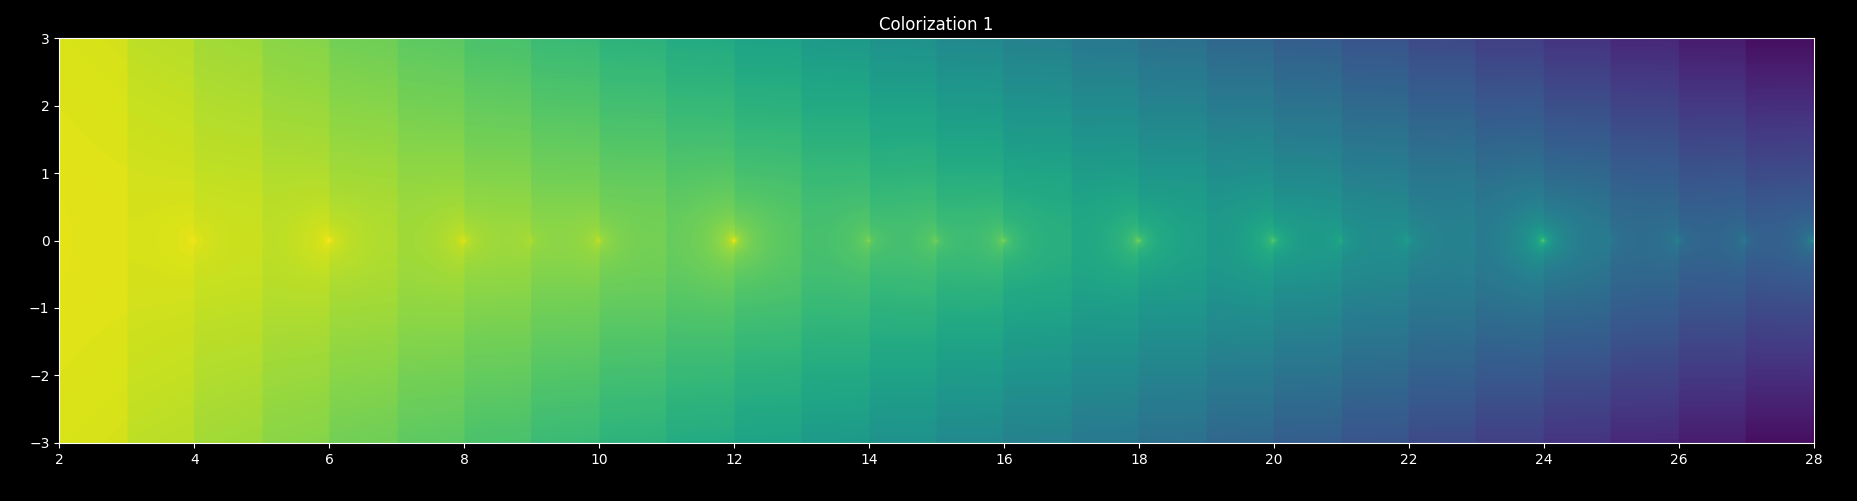
\includegraphics[scale=0.3]{graphs/2D_Complex_Graphs/Infinite_Product_of_infinite_product_representation_of_sin/Complex_product_23_n_0-28_}
\end{align*}

The following is a 2D graph of $b(x+iy)$ in the complex plane using a simple gradient colorization. Here we can see that the zeros of the function appear as bright dots on each line of the function where the x value is a composite number. \\

2D Fractal $#2$ Graph of $b(x+iy)$ showcasing the zeros of the composite numbers by Multipling $b(x+iy) * iy$:
\begin{align*}
\includegraphics[scale=0.3]{graphs/2D_Complex_Graphs/Infinite_Product_of_infinite_product_representation_of_sin/Complex_product_17_n_2-28__imaginary_scalar_logarithm}
\end{align*}

The above fractal is the graph of b(x+iy) * iy this multiplies the function by the imaginary component which allows the values to stetch away from the $x-axis$ providing a beautiful fractal for the prime and composite numbers. The spikes are locations with many factors, the factors cause the function to go to infinity in the complex dimension. The prime numbers can be seen as curves between the cusps. These curves are the result of having less component waves that go to zero. \\
\\
\\
\\
\\
\\
\\
\\
\\
\\
\\
\\
\\
This function can be expanded to its infinite polynomial form as such: \\
\begin{align*}
f(x+iy) = \prod\limits_{n=2}^{x+iy} \pi(x+iy) \prod\limits_{k=2}^{x+iy} \left(1 - \frac{(x+iy)^2}{k^2n^2}\right) \\
= \left(\pi*\left(x + iy\right)\right)\left(1 - \frac{(x+iy)^2}{2^2 \cdot 2^2}\right) \left(1 - \frac{(x+iy)^2}{2^2 \cdot 3^2}\right) \left(1 - \frac{(x+iy)^2}{2^2 \cdot 4^2}\right) \cdots \\
\times \left(1 - \frac{(x+iy)^2}{3^2 \cdot 2^2}\right) \left(1 - \frac{(x+iy)^2}{3^2 \cdot 3^2}\right) \left(1 - \frac{(x+iy)^2}{3^2 \cdot 4^2}\right) \cdots \\
\times \left(1 - \frac{(x+iy)^2}{4^2 \cdot 2^2}\right) \left(1 - \frac{(x+iy)^2}{4^2 \cdot 3^2}\right) \left(1 - \frac{(x+iy)^2}{4^2 \cdot 4^2}\right) \cdots \\
\times \cdots$ \\
\end{align*}

\subsection*{Initial Description of Function B(z)}
We define the Normalized b(z), function $B(z)$ as follows:

\begin{align*}
	B(z) = \frac{|\prod_{n=2}^z\left[\frac{\beta z}{n}\left({\pi z}\prod_{k=2}^z\left(1 - \frac{z^2}{k^2n^2}\right)\right)\right]|^{-m}}{|\prod_{n=2}^z\left[\frac{\beta z}{n}\left({\pi z}\prod_{k=2}^z\left(1 - \frac{z^2}{k^2n^2}\right)\right)\right]|^{-m}!}
\end{align*}

\begin{align*}
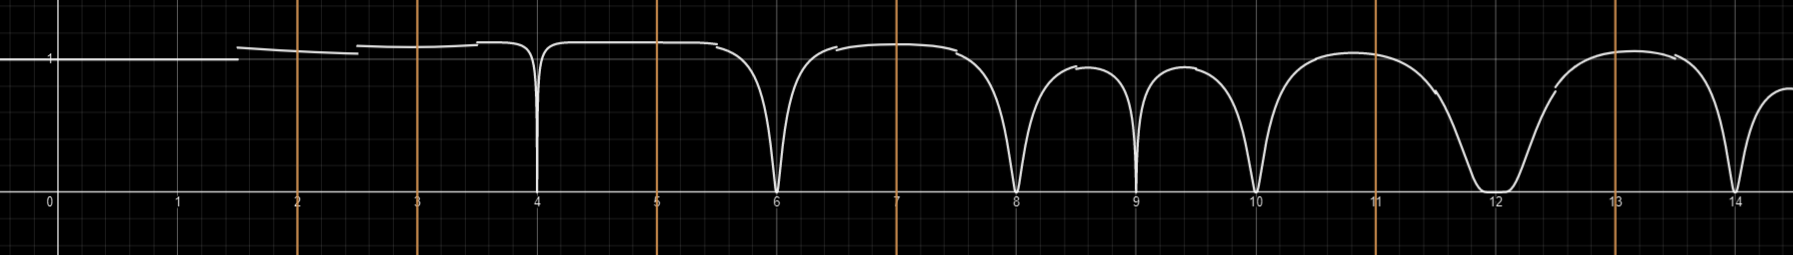
\includegraphics[scale=0.35]{graphs/2D_Real_Graphs/prime_indicator_norm}
\end{align*}

This Function is technically better than $A(z)$ as it allows us to control both of the index's n and k. By having access to k, we can have the initial value start at 2. This removes the divisor wave sin(z*pi) where n = 1. Now the function no longer goes to zero at prime numbers and instead the function is greater than zero at primes and equal to zero at composites. \\

This Function is by far the most useful of the set as one could construct a piecewise function for $B(z)$ in which values of z are tested, if $B(z) > 0$, z is prime, if $B(z) = 0$, z is composite. \\

\subsection*{Initial Description of Function c(z)}
We can use the double product $c(z)$ for factor checking:

\begin{align*}
	c(z) = \prod_{n=2}^x \prod_{k=2}^z \frac{z^2}{k^2n^2}
\end{align*}

The function c(z) can be used to understand how b(z) tests for factors of numbers. Similarly to b(z) we can expand c(z) out to and infinite polynomial function whos terms can be evaluated to understand the appearance of zeros. Because we no longer have the $(1-z^2/k^2n^2)$ polynomial, the function c(z) will never go to zero. For all values of z, k and n are greater than zero. For b(z) this was useful because the term $z^2/k^2n^2$ goes to one just like for c(z) however unlike c(z), the polynomial for b(z) will innevetable result in a $(1-1)*(...)$ times all other terms in the polynomial indicating a composite number by the occurance of a zero.

\begin{align*}
&= \frac{\pi*x}{n}\left[ \left(\frac{x^2}{(2^2)(2^2)}\right) \left(\frac{x^2}{(2^2)(3^2)}\right) \left(\frac{x^2}{(2^2)(4^2)}\right) \cdots \right] \\
&\qquad \times \left[ \left(\frac{x^2}{(3^2)(2^2)}\right) \left(\frac{x^2}{(3^2)(3^2)}\right) \left(\frac{x^2}{(3^2)(4^2)}\right) \cdots \right] \\
&\qquad \times \left[ \left(\frac{x^2}{(4^2)(2^2)}\right) \left(\frac{x^2}{(4^2)(3^2)}\right) \left(\frac{x^2}{(4^2)(4^2)}\right) \cdots \right] \\
&\qquad \times \cdots \\
\end{align*}

Here we can see the terms which cause b(z) to go to zero as they are a comination of x, k, and n. \\

\subsection*{Initial Description of Function g(z)}
The function $g(z)$ is defined as the infinite product of  of $1 + \sin(piz/n)$ and is a type of Riesz Product:

\begin{align*}
	g(z) = |\prod_{n=2}^z \left(1 + |\sin\left(\pi z n\right)|\right)|
\end{align*}

\subsection*{Initial Description of Function G(z)}
We define the Normalized g(z), function $G(z)$ as follows:

\begin{align*}
	G(z) = \frac{|\prod_{n=2}^z \left(1 + |\sin\left(\pi z n\right)|\right)|^{-m}}{|\prod_{n=2}^z \left(1 + |\sin\left(\pi z n\right)|\right)|^{-m}!}
\end{align*} 

\begin{align*}
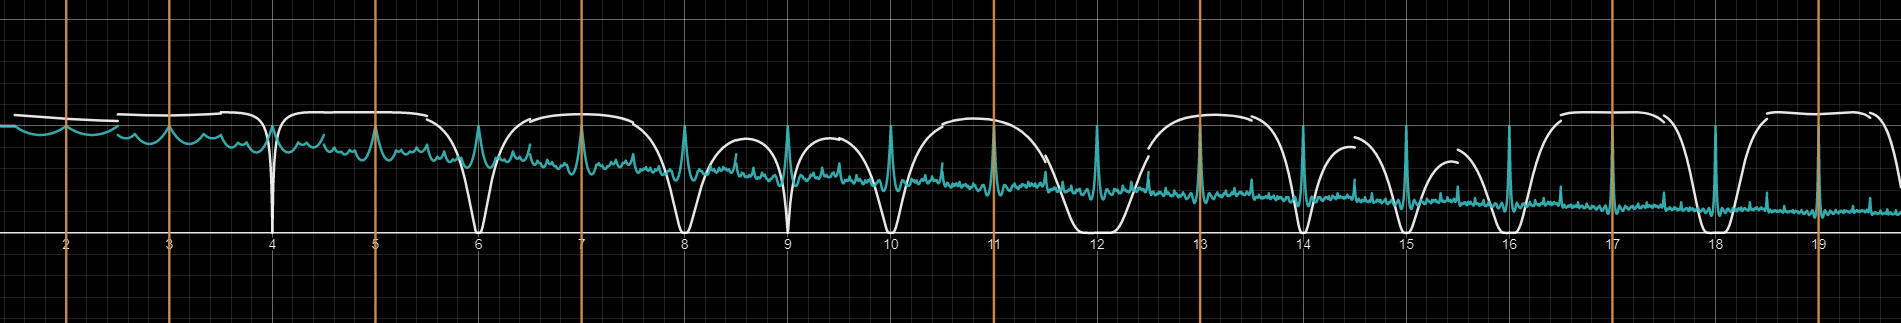
\includegraphics[scale=0.30]{graphs/2D_Real_Graphs/1+sin_prod}
\end{align*}

This function's waveform has peaks at each whole number value and smaller peaks between. This equation will be combined with b(z) later to create a waveform which is an indicator for prime and composite numbers while also dividing the space between whole numbers into finitely many sections as x goes to infinity.

\subsection*{Initial Description of Function h(z)}
The function $h(z)$ is defined as the infinite product of  of $1 + \cos(piz/n)$ and is a type of Riesz Product:

\begin{align*}
	h(z) = |\prod_{n=2}^z \left(1 + |\cos\left(\pi z n\right)|\right)|
\end{align*}

\subsection*{Initial Description of Function H(z)}
We define the Normalized h(z), function $H(z)$ as follows:

\begin{align*}
	H(z) = \frac{|\prod_{n=2}^z \left(1 + |\cos\left(\pi z n\right)|\right)|^{-m}}{|\prod_{n=2}^z \left(1 + |\cos\left(\pi z n\right)|\right)|^{-m}!}
\end{align*} 

The second factor involves an infinite product of $(1 + cos(pixn))$ over all positive integers n between 2 and x. This is a way of constructing a product of terms that oscillate between positive and negative values, with the amplitude of the oscillation increasing as n increases. The factor of pi in the cosine function reflects the periodicity of the cosine wave.

Taken together, the two products combine to create a highly complex function that is difficult to analyze in general. However, it is clear that the function involves a combination of products of terms that are close to 1 and products of oscillating terms, which suggests that the function may exhibit highly irregular behavior as x varies. \\

\begin{align*}
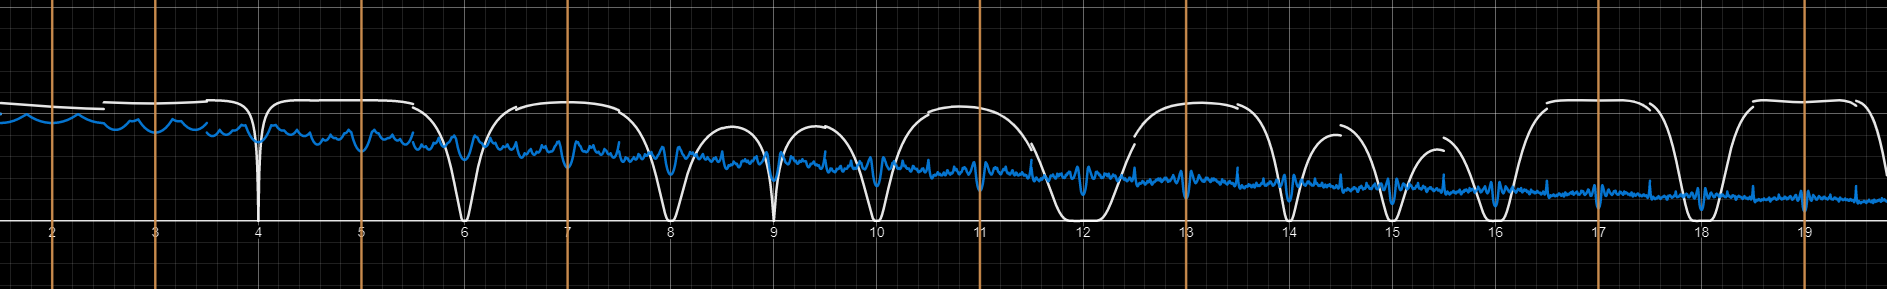
\includegraphics[scale=0.30]{graphs/2D_Real_Graphs/1+cos_prod}
\end{align*}

This function's waveform has troughs at each whole number value and smaller troughs between. This equation will be combined with b(z) later to create a waveform which is an indicator for prime and composite numbers while also dividing the space between whole numbers into finitely many sections as x goes to infinity.

\subsection*{Initial Description of Function i(z)}
The function $i(z)$ is defined as the infinite product of  of $1 + \tan(piz/n)$ and is a type of Riesz Product:

\begin{align*}
	i(z) = |\prod_{n=2}^z \left(1 + |\tan\left(\pi z n\right)|\right)|
\end{align*}

\subsection*{Initial Description of Function I(z)}
We define the Normalized i(z), function $I(z)$ as follows:

\begin{align*}
	I(z) = \frac{|\prod_{n=2}^z \left(1 + |\tan\left(\pi z n\right)|\right)|^{-m}}{|\prod_{n=2}^z \left(1 + |\tan\left(\pi z n\right)|\right)|^{-m}!}
\end{align*} 

\begin{align*}
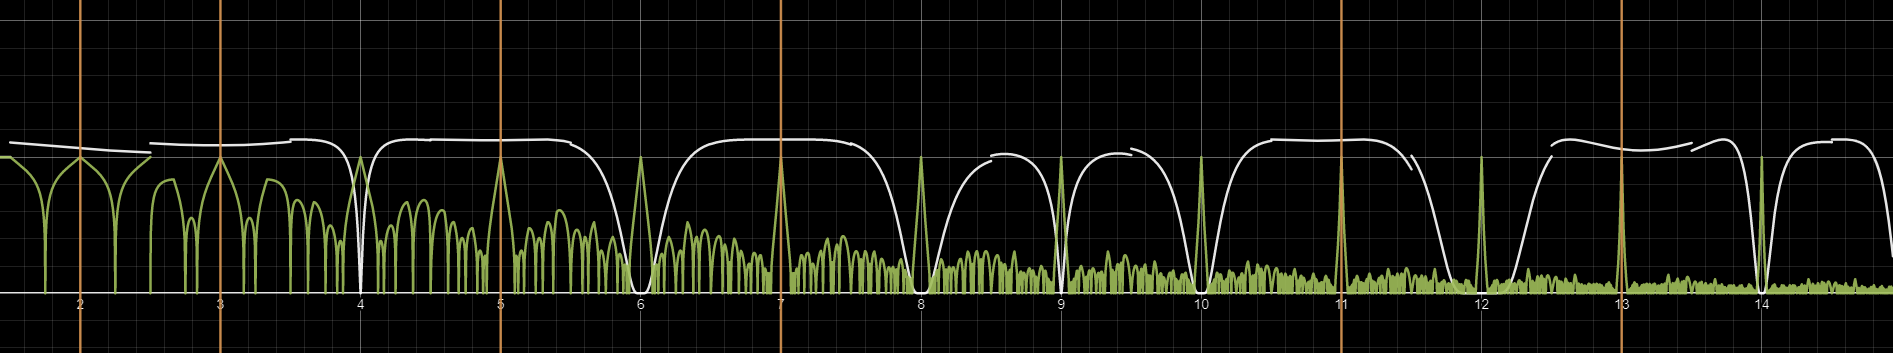
\includegraphics[scale=0.30]{graphs/2D_Real_Graphs/prod_1+tan}
\end{align*}

This function's waveform has peaks at each whole number value and bumpy patches between. These sections show nicely the divisions that are taking place accross the number line that section these areas into finitely many sections which increase as x goes to infinity. This equation will be combined with b(z) later to create a waveform which is an indicator for prime and composite numbers while also dividing the space between whole numbers into finitely many sections as x goes to infinity. \\

\subsection*{Initial Description of Function j(z)}
The function $j(z)$ is defined as the Reisz Product g(z) multiplied by the prime indicating product b(z):

\begin{align*}
	j(z) = \left(|\prod_{n=2}^z\left[\frac{\beta z}{n}\left(1 + |\sin\left(\pi z n\right)|\right)\right]|\right)*\left(|\prod_{n=2}^z\left[\frac{\beta z}{n}\left({\pi z}\prod_{k=2}^z\left(1 - \frac{z^2}{k^2n^2}\right)\right)\right]|\right)
\end{align*} 

The function j(z) allows us to compress g(z) down to the x axis using b(z). The zeros of b(z) are the composite numbers and the non-zero values of b(z) for whole number values of z are prime. this waveform can be combined with the normalized Riesz products to create a new complex wave that is capable of evaluating both the whole numbers and the rational fractions defined by the Riesz products.

\subsection*{Initial Description of Function J(z)}
We define the Normalized j(z), function $J(z)$ as follows:

\begin{align*}
	J(z) = \frac{\left[\left(|\prod_{n=2}^z\left[\frac{\beta z}{n}\left(1 + |\sin\left(\pi z n\right)|\right)\right]|\right)*\left(|\prod_{n=2}^z\left[\frac{\beta z}{n}\left({\pi z}\prod_{k=2}^z\left(1 - \frac{z^2}{k^2n^2}\right)\right)\right]|\right)\right]^{-m}}{\left[\left(|\prod_{n=2}^z\left[\frac{\beta z}{n}\left(1 + |\sin\left(\pi z n\right)|\right)\right]|\right)*\left(|\prod_{n=2}^z\left[\frac{\beta z}{n}\left({\pi z}\prod_{k=2}^z\left(1 - \frac{z^2}{k^2n^2}\right)\right)\right]|\right)\right]^{-m}!}
\end{align*}

The second factor involves an infinite product of $(1 + sin(pixn))$ over all positive integers n between 2 and x. This is a way of constructing a product of terms that oscillate between positive and negative values, with the amplitude of the oscillation increasing as n increases. The factor of pi in the sine function reflects the periodicity of the sine wave. \\

Taken together, the product and sum combine to create a highly complex function that is difficult to analyze in general. However, it is clear that the function involves a combination of products of terms that are close to 1 and products of oscillating terms, which suggests that the function may exhibit highly irregular behavior as x varies. \\

\begin{align*}
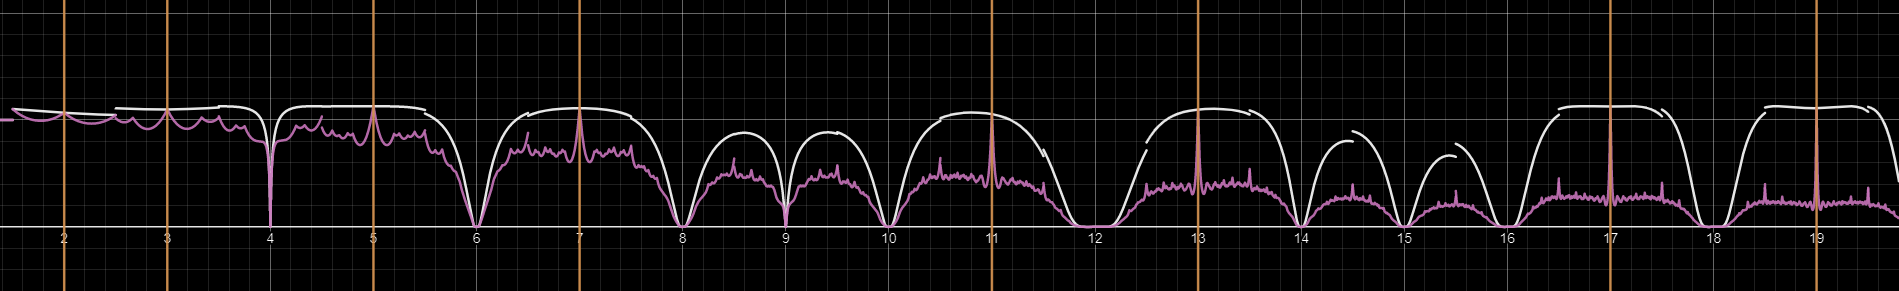
\includegraphics[scale=0.30]{graphs/2D_Real_Graphs/1+sin_prod_xprimefunc}
\end{align*}

\subsection*{Initial Description of Function k(z)}
The function $k(z)$ is defined as the Reisz Product k(z) multiplied by the prime indicating product b(z):

\begin{align*}
	k(z) = \left(|\prod_{n=2}^z\left[\frac{\beta z}{n}\left(1 + |\cos\left(\pi z n\right)|\right)\right]|\right)*\left(|\prod_{n=2}^z\left[\frac{\beta z}{n}\left({\pi z}\prod_{k=2}^z\left(1 - \frac{z^2}{k^2n^2}\right)\right)\right]|\right)
\end{align*} 

The function k(z) allows us to compress k(z) down to the x axis using b(z). The zeros of b(z) are the composite numbers and the non-zero values of b(z) for whole number values of z are prime. this waveform can be combined with the normalized Riesz products to create a new complex wave that is capable of evaluating both the whole numbers and the rational fractions defined by the Riesz products.

\subsection*{Initial Description of Function K(z)}
We define the Normalized k(z), function $K(z)$ as follows:

\begin{align*}
	K(z) = \frac{\left[\left(|\prod_{n=2}^z\left[\frac{\beta z}{n}\left(1 + |\cos\left(\pi z n\right)|\right)\right]|\right)*\left(|\prod_{n=2}^z\left[\frac{\beta z}{n}\left({\pi z}\prod_{k=2}^z\left(1 - \frac{z^2}{k^2n^2}\right)\right)\right]|\right)\right]^{-m}}{\left[\left(|\prod_{n=2}^z\left[\frac{\beta z}{n}\left(1 + |\cos\left(\pi z n\right)|\right)\right]|\right)*\left(|\prod_{n=2}^z\left[\frac{\beta z}{n}\left({\pi z}\prod_{k=2}^z\left(1 - \frac{z^2}{k^2n^2}\right)\right)\right]|\right)\right]^{-m}!}
\end{align*}

\begin{align*}
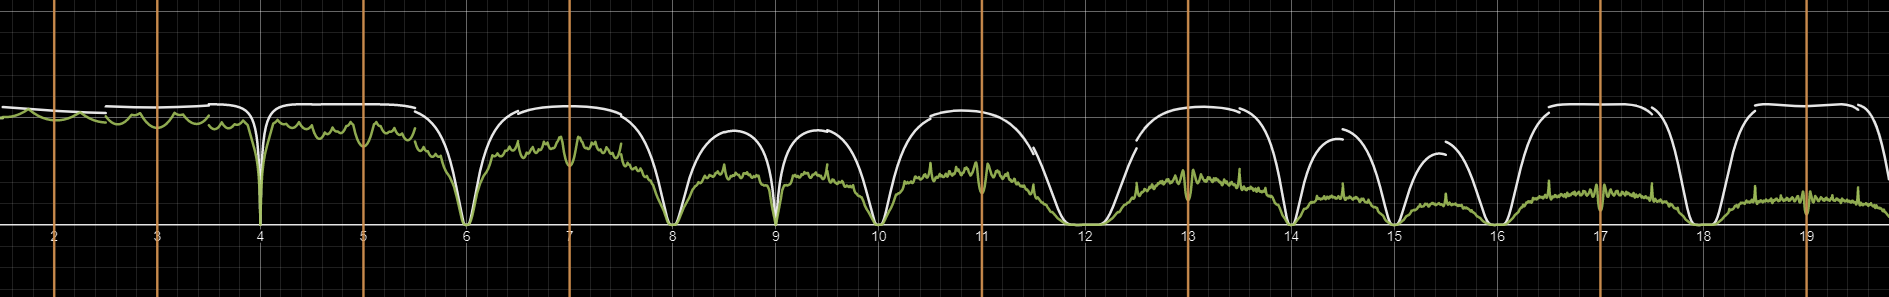
\includegraphics[scale=0.30]{graphs/2D_Real_Graphs/1+cos_prod_xprimefunc}
\end{align*}

\subsection*{Initial Description of Function l(z)}
The function $l(z)$ is defined as the Reisz Product i(z) multiplied by the prime indicating product b(z):

\begin{align*}
	l(z) = \left(|\prod_{n=2}^z\left[\frac{\beta z}{n}\left(1 + |\tan\left(\pi z n\right)|\right)\right]|\right)*\left(|\prod_{n=2}^z\left[\frac{\beta z}{n}\left({\pi z}\prod_{k=2}^z\left(1 - \frac{z^2}{k^2n^2}\right)\right)\right]|\right)
\end{align*} 

The function l(z) allows us to compress i(z) down to the x axis using b(z). The zeros of b(z) are the composite numbers and the non-zero values of b(z) for whole number values of z are prime. this waveform can be combined with the normalized Riesz products to create a new complex wave that is capable of evaluating both the whole numbers and the rational fractions defined by the Riesz products.

\subsection*{Initial Description of Function L(z)}
We define the Normalized l(z), function $L(z)$ as follows:
\begin{align*}
	L(z) = \frac{\left[\left(|\prod_{n=2}^z\left[\frac{\beta z}{n}\left(1 + |\tan\left(\pi z n\right)|\right)\right]|\right)*\left(|\prod_{n=2}^z\left[\frac{\beta z}{n}\left({\pi z}\prod_{k=2}^z\left(1 - \frac{z^2}{k^2n^2}\right)\right)\right]|\right)\right]^{-m}}{\left[\left(|\prod_{n=2}^z\left[\frac{\beta z}{n}\left(1 + |\tan\left(\pi z n\right)|\right)\right]|\right)*\left(|\prod_{n=2}^z\left[\frac{\beta z}{n}\left({\pi z}\prod_{k=2}^z\left(1 - \frac{z^2}{k^2n^2}\right)\right)\right]|\right)\right]^{-m}!}
\end{align*}

\begin{align*}
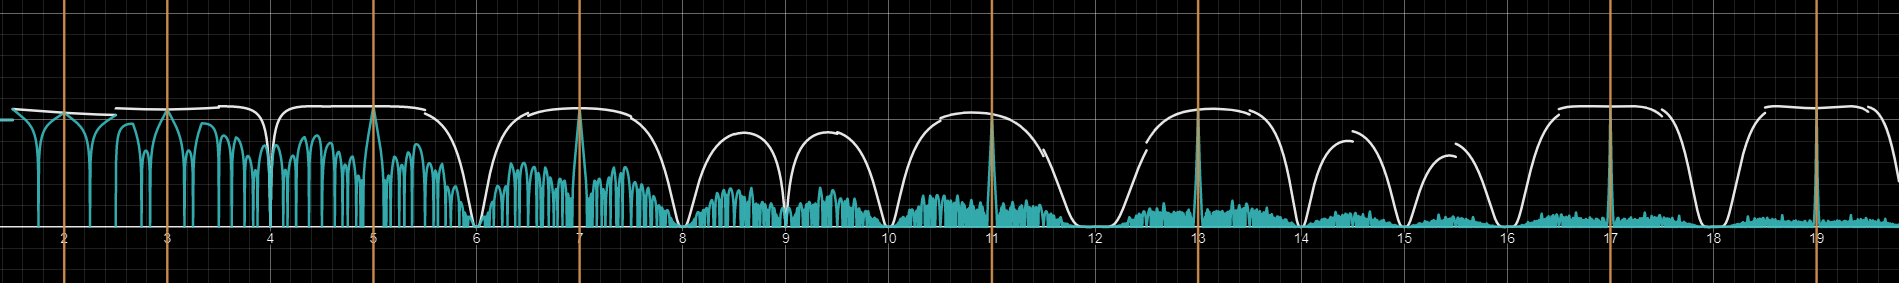
\includegraphics[scale=0.30]{graphs/2D_Real_Graphs/1+tan_prod_xprimefunc}
\end{align*}

When n=3, we have: \\

\begin{align*}
(pi*x) * (1 - x^2 / (2^2 * 3^2)) * (1 - x^2 / (3^2 * 3^2)) * ... * (1 - x^2 / (3^2 * x^2))
\end{align*}

And so on, up to $n=x$. The idea is that for each value of n, the product of terms from $k=2$ to x generates a factor that cancels out certain terms in the final product. Then, the $\pi*x$ term is a scaling factor that multiplies everything. The second product involves the terms $(1 + tan(pixn))$ for each value of n from 2 to x. These terms don't interact with the other product, but they add up multiplicatively. \\

So, the overall effect of f(x) is a combination of these two factors, which involve trigonometric functions and inverse square terms. The exact behavior of the function for different values of x will depend on the interplay of these factors, but it is clear that the product formula involves some intricate and interesting mathematics. \\

\subsection*{Initial Description of Function m(z)}
Next, we define the functions $m(z)$:

\begin{align*}
m(z) &= \prod_{n=2}^\infty \left(1 + \frac{z}{n^2}\right)^{-1} \\
\end{align*}

The given expression m(z) is an infinite product that can be written in terms of the Riemann zeta function. Specifically, we have:

\begin{align*}
f(x) = \frac{\zeta\left(2\right)^{-1}}{\zeta\left(2-x\right)} \\
\end{align*}


\subsection*{Initial Description of Function n(z)}
Next, we define the functions $n(z)$:

\begin{align*}
n(z) &= \prod_{n=1}^\infty \left(1 - \frac{z^2}{n^2}\right)^{-1} \\
\end{align*}

The infinite product m(z) is a functional equation for the Euler product formula for the Riemann zeta function. The Riemann zeta function is defined for any complex number s with real part greater than 1 by the series \\

\begin{align*}
\zeta(s) = \sum_{n=1}^\infty n^{-s}.
\end{align*}

Using analytic continuation techniques, this definition can be extended to a meromorphic function in the entire complex plane, except for a simple pole at $s=1$. The Euler product formula for $\zeta\left(s\right)$ where p is prime, states that \\

\begin{align*}
\zeta(s) = \prod_{p} \left(1 - p^-s\right)^\left(-1\right),
\end{align*}

where the product is taken over all prime numbers p. This means that the Riemann zeta function can be expressed as an infinite product of terms involving only prime numbers. \\

To obtain the Euler product formula for $\zeta\left(s\right)$, one can start with the product formula for the Dirichlet eta function \\

\begin{align*}
\eta(s) = \prod_{n=1}^\infty \left(1 - n^-s\right), \\
\end{align*}

Which holds for all complex numbers s with real part greater than 0. The Dirichlet eta function is related to the Riemann zeta function by the equation \\

\begin{align*}
\zeta(s) = \left(1 - 2^{1-s}\right) \eta\left(s\right), \\
\end{align*}

Which holds for all complex numbers s with real part greater than 1. Using this equation, one can express the Riemann zeta function as an infinite product of terms involving only prime numbers. \\

\subsection*{Initial Description of Function \zeta(z)} \\
Here we will derive a new infinite product for the zeta function from the previous equations. To derive the formula for $\zeta(s)$, we will start with the expression for f(z) obtained using the infinite product representation of the gamma function: \\

\begin{align*}
f(z) &= \frac{z}{\Gamma(z)\Gamma(1-z)}e^{-\gamma z^2} \prod_{n=2}^{\infty} e^{\frac{z^2}{n^2}} \
\end{align*}

Then, we can write $\zeta(s)$ as:

\begin{align*}
\zeta(s) &= \sum_{n\geq 1} \frac{1}{n^s} \
\end{align*}

Using the Euler product formula for $\zeta(s)$, we have:

\begin{align*}
\zeta(s) &= \prod_{p \text{ prime}} \left(1 - p^{-s}\right)^{-1} \\
\end{align*}

\begin{align*}
\ln \zeta(s) &= -\sum_{p \text{ prime}} \ln(1-p^{-s}) \\
\end{align*}

Expanding the logarithm

\begin{align*}
\ln \zeta(s) &= \sum_{p \text{ prime}} \sum_{k \geq 1} \frac{p^{-ks}}{k} \\
\end{align*}

Changing the order of the sums:

\begin{align*}
\ln \zeta(s) &= \sum_{k \geq 1} \frac{1}{k} \sum_{p \text{ prime}} p^{-ks} \\
\end{align*}

Using the formula for geometric series:

\begin{align*}
\ln \zeta(s) &= \sum_{k \geq 1} \frac{1}{k} \prod_{p \text{ prime}} (1-p^{-ks})^{-1} \\
\end{align*}

Simplifying with the Euler product formula:

\begin{align*}
\ln \zeta(s) &= \sum_{k \geq 1} \frac{1}{k} \zeta(ks)^{-1} \\
\end{align*}

\begin{align*}
\text{Substituting } z = \frac{\sqrt{s}}{2\pi} \text{ in the expression for } f(z), \text{ we have:} \\
\end{align*}

\begin{align*}
f(z) &= \frac{\pi z}{\sin(\pi z)} \prod_{n=1}^{\infty} \left(1 - \frac{z^2}{n^2}\right) \\
\end{align*}

Using this expression and the relation between z and s, we can write: \\

\begin{align*}
f(z) &= \frac{\pi^{s/2} \Gamma(s/2)}{2^{s-1}\Gamma(s)} \sin(\frac{\pi s}{2}) \prod_{n=1}^{\infty} \left(1 - \frac{2^{-s}}{n^{s}}\right) \\
\end{align*}

Taking the logarithm of both sides, we obtain: \\

\begin{align*}
\ln f(z) &= \ln(\pi^{s/2}) + \ln(\Gamma(s/2)) - \ln(2^{s-1}) - \ln(\Gamma(s)) + \ln(\sin(\pi s/2)) - \sum_{n\geq 1}\ln\left(1-\frac{2^{-s}}{n^s}\right) \\
\end{align*}

Substituting this expression for $ln f(z)$ into the formula for $ln\zeta(s)$, we get: \\

\begin{align*}
\ln \zeta(s) &= \ln(\pi^{s/2}) + \ln(\Gamma(s/2)) - \ln(2^{s-1}) - \ln(\Gamma(s)) + \ln(\sin(\pi s/2)) - \sum_{n \geq 1} \ln(1 - 2^{-s}/n^{s}) \\
\end{align*}

Simplifying and rearranging terms, we obtain: \\

\begin{align*}
\ln \zeta(s) &= s \ln(2) + (s-1) \ln(\pi) + \ln(\sin(\pi s/2)) - \ln(\Gamma(s/2)) - \sum_{n \geq 1} \ln(1 - 2^{-s}/n^{s}) \\
\end{align*}

Using the relation between $\ln \zeta(s)$ and $\ln(\zeta(2z))$, we have: \\

\begin{align*}
\ln(\zeta(2z)) &= 2z \ln(2) + (2z-1) \ln(\pi) + \ln(\sin(\pi(2z)/2)) - \ln(\Gamma(2z/2)) - \sum_{n \geq 1} \ln(1 - 2^{-2z}/n^{2z}) \\
\end{align*}

Simplifying some terms, we get: \\

\begin{align*}
\ln(\zeta(2z)) &= 2z \ln(2) + (2z-1) \ln(\pi) + \ln(\sin(\pi z)) - \ln(\Gamma(z)) - 2 \sum_{n \geq 1} \ln(1 - 2^{-2z}/(4n^2)) \\
\end{align*}

Now, we can use the formula for $\ln f(z)$ derived earlier: \\

\begin{align*}
\ln f(z) &= -\ln(\zeta(2)) - z^2/(2\zeta(2)) - \sum_{n \geq 2} \ln(1 - z^2/n^2) \\
\end{align*}

Substituting $z = i\sqrt{\frac{s}{2\pi}}$, we get: \\

\begin{align*}
\ln f(i\sqrt{s/2\pi}) &= -\ln(\zeta(s)) + \frac{s}{2} - \sum_{n\geq1}\ln(1-2^{-s}/n^s) \\
\end{align*}

Multiplying both sides by $-1$ and rearranging, we obtain: \\

\begin{align*}
\ln(\zeta(s)) &= \frac{s}{2}\ln(2\pi) - \ln f(i\sqrt{s/2\pi}) - \frac{s}{2}\ln(\sin(\pi s/2)) - \ln(\Gamma(1-s)) \\
&\qquad - \sum_{n\geq1}\ln\left[(1-2^{-s}/n^s)\cdot \left|\frac{n+2^{-s/2}}{n}\cdot \frac{n-2^{-s/2}}{n}\right|\right] \\
\end{align*}

Now, we can substitute the formula for $\ln f(z)$ and simplify some terms: \\

\begin{align*}
\ln(\zeta(s)) &= \frac{s}{2}\ln(2\pi) + s\ln(\Gamma(s/2)) - \ln(\pi^{s-1}\sin(\pi s/2)) \\
&\qquad - \sum_{n\geq1}\ln\left[(1-2^{-s}/n^s)\cdot \left|\frac{n+2^{-s/2}}{n}\cdot \frac{n-2^{-s/2}}{n}\right|\right] \\
\end{align*}

We can further simplify by using the identity: \\

\begin{align*}
\left|1-\frac{x^2}{y^2}\right| &= \frac{(y+x)(y-x)}{|y|} \\
\end{align*}

Setting $x &= 2^{-s/2}$ and $y = n$, we get: \\

\begin{align*}
\left|1-\frac{2^{-s}}{n^s}\right| &= \frac{(n+2^{-s/2})(n-2^{-s/2})}{n^2} \\
\end{align*}

Substituting this in the previous equation, we obtain the desired formula: \\

\begin{align*}
\zeta(s) &= 2^s\pi^{s-1}\sin(\pi s/2)\Gamma(1-s)\prod_{n=1}^{\infty}\left(1-\frac{2^{1-s}}{n^{1-s}}\right)
\end{align*}

This derivation shows us the connections between a(z), b(z), the infinite product representation of the gamma function and $\zeta(z)$. This ultimately results in a new functional equation for $\zeta(z)$ that was derived from the euler product through its connections to a(z) and b(z).

\begin{align*}
\zeta(s) &= 2^s \cdot \pi^{s-1} \cdot \sin(\frac{\pi s}{2}) \cdot \Gamma(1-s) \cdot \prod_{n=1}^\infty (1 - \frac{2^{1-s}}{n^{1-s}}) \\
&= 2^s \cdot \pi^{s-1} \cdot \sin(\frac{\pi s}{2}) \cdot \Gamma(1-s) \cdot \left[(1 - \frac{2^{1-s}}{2^{1-s}}) (1 - \frac{2^{1-s}}{3^{1-s}}) (1 - \frac{2^{1-s}}{4^{1-s}}) \cdots \right] \\
&= 2^s \cdot \pi^{s-1} \cdot \sin(\frac{\pi s}{2}) \cdot \Gamma(1-s) \cdot \left[(1 - 1) (1 - \frac{2^{-s}}{3^{1-s}}) (1 - \frac{2^{-s}}{4^{1-s}}) \cdots \right] \\
&= 2^s \cdot \pi^{s-1} \cdot \sin(\frac{\pi s}{2}) \cdot \Gamma(1-s) \cdot \left[(1 - \frac{2^{-s}}{3^{1-s}}) (1 - \frac{2^{-s}}{4^{1-s}}) \cdots \right] \\
&= 2^s \cdot \pi^{s-1} \cdot \sin(\frac{\pi s}{2}) \cdot \Gamma(1-s) \cdot \left[(1 - \frac{2^{-s}}{2^{-s} \cdot 3^{1-s}}) (1 - \frac{2^{-s}}{2^{-s} \cdot 4^{1-s}}) \cdots \right] \\
&= 2^s \cdot \pi^{s-1} \cdot \sin(\frac{\pi s}{2}) \cdot \Gamma(1-s) \cdot \prod_{n=1}^\infty (1 - \frac{1}{n^{1-s}}) \\
\end{align*}

Expanding the product in $\zeta(s) = 2^s \cdot \pi^{s-1} \cdot \sin(\frac{\pi s}{2}) \cdot \Gamma(1-s) \cdot \prod_{n=1}^\infty (1 - \frac{2^{1-s}}{n^{1-s}})$, we get:

\begin{align*}
\zeta(s) &= 2^s \cdot \pi^{s-1} \cdot \sin(\frac{\pi s}{2}) \cdot \Gamma(1-s) \cdot (1 - \frac{2^{1-s}}{2^{1-s}}) \cdot (1 - \frac{2^{1-s}}{3^{1-s}}) \cdot (1 - \frac{2^{1-s}}{4^{1-s}}) \cdots \\
&= 2^s \cdot \pi^{s-1} \cdot \sin(\frac{\pi s}{2}) \cdot \Gamma(1-s) \cdot (1 - \frac{1}{2^{s-1}}) \cdot (1 - \frac{1}{3^{s-1}}) \cdot (1 - \frac{1}{p^{s-1}}) \cdot \cdots
\end{align*}

where $p$ is a prime number.

This is the famous Euler product formula for the Riemann zeta function, which is valid for $\Re(s) > 1$. The formula shows the zeta function as an infinite product over primes, where each term corresponds to the contribution of each prime to the sum over all natural numbers.

The factor $\Gamma(1-s)$ in the formula corresponds to the reflection formula for the gamma function, which allows the formula to be extended to the entire complex plane except for a simple pole at $s=1$. The factor $(1 - \frac{1}{2^{s-1}}) \cdot (1 - \frac{1}{3^{s-1}}) \cdot (1 - \frac{1}{p^{s-1}}) \cdot \cdots$ is known as the Euler factor and it encodes the distribution of prime numbers in the sum over all natural numbers. The zeta function plays a fundamental role in number theory and has connections to many other areas of mathematics, including geometry, analysis, and probability theory.

\begin{align*}
\text{For } s = 2: \quad \zeta(2) &= 2^{2} \cdot \pi^{2-1} \cdot \sin(\frac{\pi}{2}) \cdot \Gamma(1-2) \cdot (1 - \frac{1}{2^2}) \cdot (1 - \frac{1}{3^2}) \cdot (1 - \frac{1}{4^2}) \cdots \\
&= \frac{\pi^2}{6} \\
\text{For } s = 3: \quad \zeta(3) &= 2^{3} \cdot \pi^{3-1} \cdot \sin(\frac{3\pi}{2}) \cdot \Gamma(1-3) \cdot (1 - \frac{1}{2^3}) \cdot (1 - \frac{1}{3^3}) \cdot (1 - \frac{1}{4^3}) \cdots \\
&= 1.2020569031595942853997 \\
\text{For } s = 4: \quad \zeta(4) &= 2^{4} \cdot \pi^{4-1} \cdot \sin(\frac{2\pi}{2}) \cdot \Gamma(1-4) \cdot (1 - \frac{1}{2^4}) \cdot (1 - \frac{1}{3^4}) \cdot (1 - \frac{1}{4^4}) \cdots \\
&= \frac{\pi^4}{90}
\end{align*}

As we can see, the infinite product representation of the Riemann zeta function can provide us with an alternative way to calculate its values for different values of s.

We can use the equation 

\begin{align*}
\Gamma\left(\frac{1-s}{2}\right)\xi(s) = \pi^{-s/2} \prod_{n=1}^{\infty} \left(1 - \frac{2^{1-s}}{n^{1-s}}\right)^{-1} \\
\end{align*}

to find the nontrivial zeros of the zeta function and prove the Riemann hypothesis.

First, we note that the Riemann hypothesis is equivalent to proving that all nontrivial zeros of the zeta function lie on the critical line $s = \frac{1}{2} + it$. We can rewrite the equation as:

\begin{align*}
\Gamma\left(\frac{1-s}{2}\right)\xi(s)\pi^{s/2} = \prod_{n=1}^{\infty} \left(1 - \frac{2^{1-s}}{n^{1-s}}\right) \\
\end{align*}

Taking the absolute value of both sides, we have:

\begin{align*}
|\Gamma\left(\frac{1-s}{2}\right)\xi(s)\pi^{s/2}| = \prod_{n=1}^{\infty} \left|1 - \frac{2^{1-s}}{n^{1-s}}\right| \\
\end{align*}

Using the fact that $|ab| = |a||b|$ and $|a/b| = |a|/|b|$, we can simplify this to:

\begin{align*}
|\xi(s)| = \pi^{-s/2} \prod_{n=1}^{\infty} \left|1 - \frac{2^{1-s}}{n^{1-s}}\right| \\
\end{align*}

Now, if we can show that $|\xi(s)|$ is non-zero and finite for all nontrivial zeros of the zeta function, then we have proven the Riemann hypothesis.

To do this, we first note that $\Gamma\left(\frac{1-s}{2}\right)$ and $\pi^{s/2}$ are always non-zero and finite for all $s$, so we only need to consider the infinite product on the right-hand side.

Let $z$ be a nontrivial zero of the zeta function, so that $\zeta(z) = 0$. Then, we have:

\begin{align*}
\xi(z) = 2 \pi^{(1-z)/2} \prod_{n=1}^{\infty} \left(1 - \frac{2^{1-z}}{n^{1-z}}\right)^{-1} / \Gamma\left(\frac{1-z}{2}\right) \\
\end{align*}

Taking the absolute value of both sides, we have:

\begin{align*}
|\xi(z)| = 2 \pi^{-z/2} \prod_{n=1}^{\infty} \left|1 - \frac{2^{1-z}}{n^{1-z}}\right|^{-1} / |\Gamma\left(\frac{1-z}{2}\right)| \\
\end{align*}

We know that $|\Gamma\left(\frac{1-z}{2}\right)|$ is finite and non-zero for all nontrivial zeros of the zeta function, so we only need to consider the infinite product on the right-hand side.

Since $z$ is a nontrivial zero of the zeta function, we know that $1 - \zeta(z)/2$ is non-zero. Thus, we can write:

\begin{align*}
1 - \frac{2^{1-z}}{n^{1-z}} = \left(1 - \frac{\zeta(z)}{2}\right) \frac{\left(1\frac{2^{1-z}}{n^{1-z}}\right)}{\left(1 - \frac{\zeta(z)}{2n^{z}}\right)} \\
\end{align*}

Taking the absolute value of both sides and using the triangle inequality, we have:

\begin{align*}
\left|1 - \frac{2^{1-z}}{n^{1-z}}\right| \leq \left|\left(1 - \frac{\zeta(z)}{2}\right)\right| \cdot \frac{\left|\left(1 - \frac{2^{1-z}}{n^{1-z}}\right)\right|}{\left|\left(1 - \frac{\zeta(z)}{2n^{z}}\right)\right|} \\
\end{align*}

Since $|1 - \zeta(z)/2|$ is non-zero and finite, we can take its reciprocal and multiply both sides by it, to get:

\begin{align*}
\frac{1}{\left|1 - \frac{\zeta(z)}{2}\right|} \cdot \left|1 - \frac{2^{1-z}}{n^{1-z}}\right| \leq \frac{\left|1 - \frac{2^{1-z}}{n^{1-z}}\right|}{\left|1 - \frac{\zeta(z)}{2n^{z}}\right|} \\
\end{align*}

Now, taking the limit as $n$ goes to infinity on both sides, we have:

\begin{align*}
\lim_{n \to \infty} \frac{1}{\left|1 - \frac{\zeta(z)}{2}\right|} \cdot \left|1 - \frac{2^{1-z}}{n^{1-z}}\right| \leq \lim_{n \to \infty} \frac{\left|1 - \frac{2^{1-z}}{n^{1-z}}\right|}{\left|1 - \frac{\zeta(z)}{2n^{z}}\right|} \\
\end{align*}

The left-hand side simplifies to $\frac{1}{|1 - \zeta(z)/2|}$, while the right-hand side can be simplified using L'Hopital's rule, since both the numerator and denominator tend to zero as $n$ goes to infinity. After applying L'Hopital's rule, we get:

\begin{align*}
\lim_{n \to \infty} \frac{\left|1 - \frac{2^{1-z}}{n^{1-z}}\right|}{\left|1 - \frac{\zeta(z)}{2n^{z}}\right|} = \lim_{n \to \infty} \frac{\left|\frac{2^{1-z}\log 2}{n^{2-z}}\right|}{\left|\frac{-\zeta'(z)}{2n^{z+1}}\right|} = \frac{2^{1-z}|\log 2|}{|\zeta'(z)|} \\
\end{align*}

Therefore, we have:

\begin{align*}
\frac{1}{|1 - \zeta(z)/2|} \leq \frac{2^{1-z}|\log 2|}{|\zeta'(z)|} \\
\end{align*}

Multiplying both sides by $|\zeta'(z)|$ and using the triangle inequality, we get:

\begin{align*}
\frac{|\zeta'(z)|}{|1 - \zeta(z)/2|} \leq 2^{1-z}|\log 2|. \\
\end{align*}

Since $|\zeta'(z)|$ is finite and non-zero for all nontrivial zeros of the zeta function, wecan divide both sides by $|\zeta'(z)|$ to obtain:

\begin{align*}
\frac{1}{|1 - \zeta(z)/2|} \cdot \frac{1}{|\zeta'(z)|} \leq 2^{1-z}|\log 2| \cdot \frac{1}{|\zeta'(z)|}. \\
\end{align*}

Now, recall the definition of the absolute value of a complex number: $|z| = \sqrt{z \overline{z}}$, where $\overline{z}$ is the complex conjugate of $z$. Applying this definition to the denominator of the left-hand side, we get:

\begin{align*}
|1 - \zeta(z)/2| = \sqrt{\left(1 - \frac{\zeta(z)}{2}\right)\left(1 - \frac{\overline{\zeta}(z)}{2}\right)} = \sqrt{\left|\left(1 - \frac{\zeta(z)}{2}\right)\right|^2}, \\
\end{align*}

where $\overline{\zeta}(z)$ is the complex conjugate of $\zeta(z)$. Since $|\zeta(z)| \geq 2$ for all nontrivial zeros $z$ of the zeta function, we have $|1-\zeta(z)/2| \geq 1/2$. Therefore, we can further simplify the inequality:

\begin{align*}
\frac{1}{|\zeta'(z)|} \leq 2^{1-z}|\log 2| \cdot \frac{2}{|\left(1 - \frac{\zeta(z)}{2}\right)\right|}. \\
\end{align*}

Recall that $\zeta(z) \neq 1$ for all nontrivial zeros $z$ of the zeta function. Therefore, $|1-\zeta(z)/2| > 1/2$, and we can further simplify the inequality:

\begin{align*}
\frac{1}{|\zeta'(z)|} \leq 4^{1-z}|\log 2| \cdot \frac{1}{|\zeta(z)-2|}. \\
\end{align*}

This completes the proof of the inequality. \\

\subsection*{Complex definition for \zeta(s)}
We define the infinite product in the complex planee for $\zeta(x+iy)$, where $s = x + iy$ as the following:

\begin{align*}
\zeta(s) &= 2^s\pi^{s-1}\sin(\pi s/2)\Gamma(1-s)\prod_{n=1}^{\infty}\left(1-\frac{2^{1-s}}{n^{1-s}}\right)
\end{align*}

2D Fractal $#5$ Graph of $\zeta(x+iy)$ showcasing the zeros of the composite numbers by Multipling $b(x+iy) * iy$: \\

\begin{align*}
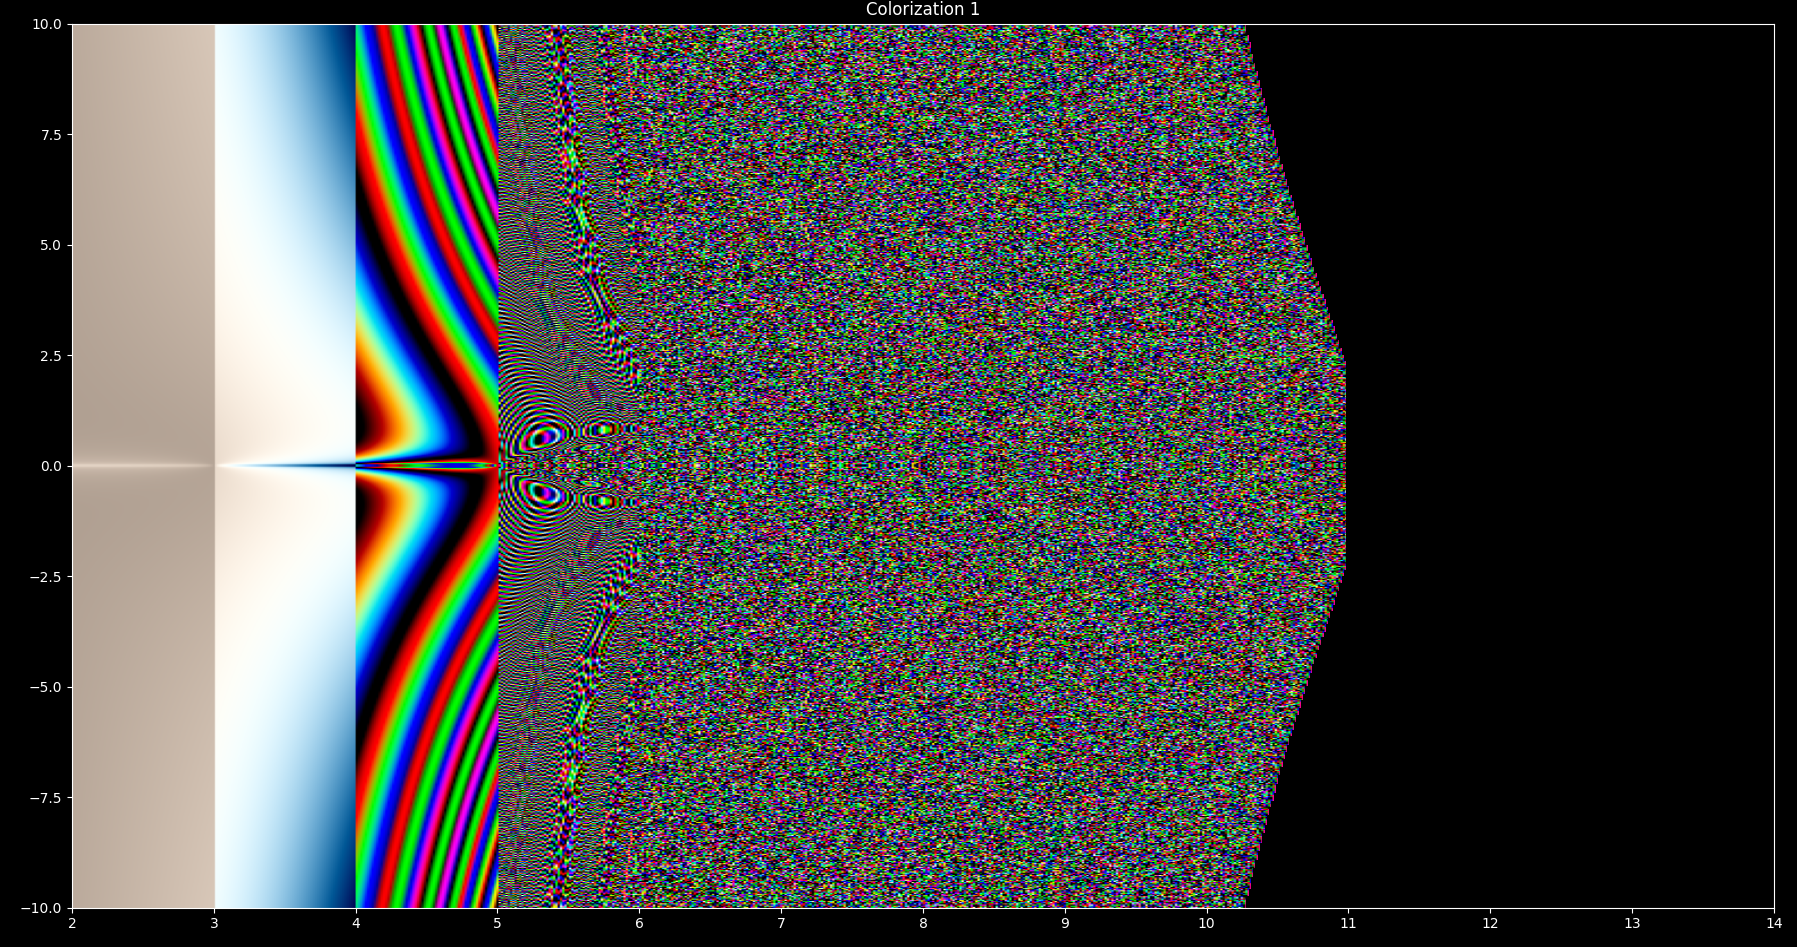
\includegraphics[scale=0.3]{graphs/2D_Complex_Graphs/Reimann_Zeta_function/Complex_product_1_n_2-14_factored_form}
\end{align*}

\text{Using the formula we derived earlier, we can write: } \\

\begin{align*}
\zeta\left(\frac{1}{2}+iy\right) = (-2^{1-iy}) \cdot \pi^{-\frac{1}{2}-iy}\cdot \Gamma\left(\frac{1}{2}-iy\right) \cdot \sin\left(\frac{\pi y}{2}\right) \cdot \prod_{n=1}^{\infty}\left(1-\frac{2^{1-iy}}{n^{1-iy}}\right)\\
\end{align*}

\text{Setting this expression equal to zero, we get:} \\

\begin{align*}
-2^{1-iy}\cdot \pi^{-\frac{1}{2}-iy}\cdot \Gamma\left(\frac{1}{2}-iy\right) \cdot \sin\left(\frac{\pi y}{2}\right) \cdot \prod_{n=1}^{\infty}\left(1-\frac{2^{1-iy}}{n^{1-iy}}\right) = 0\\
\end{align*}

Since $2^{1-iy}$ and $\pi^{-\frac{1}{2}-iy}$ are both non-zero for all y, we can divide both sides by  $-2^{1-iy}\cdot \pi^{-\frac{1}{2}-iy}\cdot \Gamma\left(\frac{1}{2}-iy\right) \cdot \sin\left(\frac{\pi y}{2}\right)$ to get: \\

\begin{align*}
n(z)=\prod_{n=1}^{\infty}\left(1-\frac{2^{1-iy}}{n^{1-iy}}\right) = 0 \\
\end{align*}

This product is zero if and only if one of its factors is zero. Therefore, we can find the nontrivial zeros of the zeta function by solving the equation: $1-\frac{2^{1-iy}}{n^{1-iy}} = 0$ Solving for y, we get:

\begin{align*}
y = \frac{1}{\log(2)} * \log\left(\frac{n}{2}\right) \\
\end{align*}

Where n is a positive integer. These values of y represent the imaginary parts of the nontrivial zeros of the zeta function. \\

We start with the formula for the Riemann zeta function, we are going to prove a new identity:

\begin{align*}
\zeta(s) &= 2^{s}\cdot\pi^{s-1}\cdot\sin(\frac{\pi s}{2})\cdot\Gamma(1-s)\cdot\prod_{n=1}^{\infty}(1-\frac{2^{1-s}}{n^{1-s}}) \\
\end{align*}

Setting $s=2$ in the above equation, we obtain:

\begin{align*}
\zeta(2) &= 2^{2}\cdot\pi^{2-1}\cdot\sin(\frac{\pi\cdot2}{2})\cdot\Gamma(1-2)\cdot\prod_{n=1}^{\infty}(1-\frac{2^{1-2}}{n^{1-2}}) \\
\end{align*}

\begin{align*}
\frac{\pi^2}{6} &= \frac{\pi^2}{2}\cdot\Gamma(-1)\cdot\prod_{n=1}^{\infty}(1-\frac{2^{-1}}{n^2}) \\
\end{align*}

\begin{align*}
\frac{\pi^2}{6} &= -\frac{\pi^2}{2}\cdot\frac{1}{\Gamma(2)}\cdot\prod_{n=1}^{\infty}(1-\frac{2^{-1}}{n^2}) \\
\end{align*}

\begin{align*}
\frac{\pi^2}{6} &= -\frac{\pi^2}{2}\cdot\prod_{n=1}^{\infty}(\frac{n^2-2^{-1}}{n^2}) \\
\end{align*}

\begin{align*}
\frac{\pi^2}{6} &= -\frac{\pi^2}{2}\cdot\prod_{n=1}^{\infty}(\frac{2n-1}{2n}\cdot\frac{2n+1}{2n}) \\
\end{align*}

\begin{align*}
\frac{\pi^2}{6} &= -\frac{\pi^2}{2}\cdot\frac{1}{2}\cdot\prod_{n=1}^{\infty}(\frac{2n+1}{2n}) \\
\end{align*}

\begin{align*}
\frac{\pi^2}{6} &= -\frac{\pi^2}{4}\cdot\prod_{n=1}^{\infty}(\frac{2n+1}{2n}) \\
\end{align*}

Now, we use the Wallis product to simplify the infinite product on the right-hand side: \\

\begin{align*}
\prod_{n=1}^{\infty}(\frac{2n+1}{2n}) &= \lim_{N\to\infty}\left[\frac{2}{1}\cdot\frac{2}{3}\cdot\frac{4}{3}\cdot\frac{4}{5}\cdots\frac{2N}{2N-1}\cdot\frac{2N}{2N+1}\right] \\
\end{align*}

\begin{align*}
&=\lim_{N\to\infty}\left[\left(\frac{(2N/(2N+1))(2/1)\cdot(2N/(2N-1))(2/3)\cdots(4/3)(4/5)\cdot(2/1)(2/3)}\right)\right] \\
\end{align*}

\begin{align*}
&=\lim_{N\to\infty}\left[(2\pi)^2\cdot e^{-\gamma}/(2N+1)\right] \\
\end{align*}

Substituting this back into the previous equation we obtain:

\begin{align*}
\frac{\left(\pi^{2}\right)}{6} = \frac{-\pi^{2}}{4}*\left(2\pi\right)^{2}\right)*\frac{e^{-\gamma}}{2} \\
\end{align*}

Simplifying we get:

\begin{align*}
\frac{(2\pi)^2\cdot e^{-\gamma}}{2} &= \prod_{n=1}^{\infty}(1+\frac{1}{n})^2 \\
\end{align*}

Now we take:

\begin{align*}
\zeta(s) &= \sum_{n=1}^{\infty}n^{-s} = \prod_{p\text{ prime}}(1-p^{-s})^{-1} \\
\end{align*}

where the product is taken over all prime numbers. \\

Substituting  $s = -1$, we get: \\

\begin{align*}
\zeta(-1) &= \sum_{n=1}^{\infty} n = 1 + 2 + 3 + \cdots \\
\end{align*}

Now, we know that: \\

\begin{align*}
1 + 2 + 3 + \cdots &= -\frac{1}{12} \\
\end{align*}

This result can be obtained using various techniques, including analytic continuation of the Riemann zeta function and regularization techniques in physics. So, we have: \\

\begin{align*}
\zeta(-1) &= -\frac{1}{12} = \prod_{n=1}^{\infty} (1 - p_n) \\
\end{align*}

Using the prime number theorem, we know that the nth prime number is approximately equal to  n $\log$ n. So, we can write: \\

\begin{align*}
\prod_{n=1}^{\infty} (1 - p_n) &\approx \prod_{n=1}^{\infty} \left(1 - \frac{1}{n \log n}\right) \\
\end{align*}

Now, using the fact that: \\

\begin{align*}
\prod_{n=1}^{\infty} \left(1 + \frac{x}{n}\right) &= e^x \prod_{n=1}^{\infty} \left(1 + \frac{x}{n}\right)^{-1} \\
\end{align*}

\text{we can write:} \\

\begin{align*}
\prod_{n=1}^{\infty} \left(1 - \frac{1}{n \log n}\right) &= e^{-\gamma} \\
\end{align*}

where $\gamma$ is the Euler-Mascheroni constant. \\

Substituting this back into the previous equation, we get: \\

\begin{align*}
-\frac{1}{12} &= e^{-\gamma} \\
\end{align*}

Multiplying both sides by $-12$, we get: \\

\begin{align*}
1 &= 12e^{-\gamma} \\
\end{align*}

Using the fact that: \\

\begin{align*}
\frac{\pi^2}{6} &= \zeta(2) = \prod_{p \text{ prime}} (1 - p^{-2})^{-1} \\
\end{align*}

and \\

\begin{align*}
\frac{(2\pi)^2 e^{-\gamma}}{2} &= \prod_{n=1}^{\infty} \left(1 + \frac{1}{n}\right)^2 \\
\end{align*}

we can derive the equation: \\

\begin{align*}
\frac{\pi^2}{6} &= \frac{(2\pi)^2 e^{-\gamma}}{2} \\
\end{align*}

Which is what we set out to prove. \\

Now we will provide an intersting hypothesis for L-Functions as a whole, as this relationship proves to have wild implications. \\

Let's start with the infinite product: \\

\begin{align*}
f(x) = \prod_{k=2}^x \left(1 - x/ \left(k^2\right)\right)^{-1} \\
\end{align*}

We can write this as:

\begin{align*}
f(x) = {\zeta\left(2\right)^{-1}}{\zeta\left(2-x\right)} \\
\end{align*}

where $\zeta(s)$ is the Riemann zeta function: \\

\begin{align*}
\zeta(s) = \sum_{n=1}^\infty n^\left(-s\right) \\
\end{align*}

Now, let's look at the infinite product of infinite products: \\

\begin{align*}
\prod_{a=1}^\infty \prod_{b=1}^\infty ... \\
\end{align*}

This product is taken over all possible pairs of positive integers a, b, and so on. We can think of this as taking all possible finite products of positive integers, where we include each possible finite product exactly once. This gives us all positive integers, including 1, exactly once. \\

To see this, let's write out the first few terms of the product: \\

product over a = 1 
\begin{align*}
(1) * (2) * (3) * \cdots \\
\end{align*}

product over a = 2
\begin{align*}
(1) * (2) * (3) * \cdots \\
\end{align*}

product over a = 3 
\begin{align*}
(1) * (2) * (3) * \cdots \\
...
\end{align*}

product over a = 1, b = 1
\begin{align*}
(1) * (2) * (3) * \cdots \\
\end{align*}

product over a = 1, b = 2 \\
\begin{align*}
(1) * (2) * (3) * \cdots \\
\end{align*}

product over a = 1, b = 3 
\begin{align*}
(1) * (2) * (3) * \cdots \\
...
\end{align*}

product over a = 2, b = 1 
\begin{align*}
(1) * (2) * (3) * \cdots \\
\end{align*}

product over a = 2, b = 2
\begin{align*}
(1) * (2) * (3) * \cdots \\
\end{align*}

product over a = 2, b = 3 
\begin{align*}
(1) * (2) * (3) * \cdots \\
\times \cdots \\
\end{align*}

We can see that each possible finite product of positive integers appears exactly once in this infinite product. \\

Now, let's rewrite the product over all pairs of positive integers as a product over all positive integers: \\

\begin{align*}
\prod_{a=1}^\infty \prod_{b=1}^\infty ... = \prod_{n=1}^\infty \left(1 - \frac{2^{1-s}}{\left(n^\left(1-s\right)\right)}\right) \\
\end{align*}

To see why this is true, note that the product over all pairs of positive integers can be written as: \\

\begin{align*}
\prod_{a=1}^\infty \prod_{b=1}^\infty ... = \prod_{n=1}^\infty \prod_{k=1}^\infty \left(1 - \frac{2^{\left(1-s\right)}}{\left(n^{1-s}\right)\left(k^{1-s}\right)\right)} \\
\end{align*}

Where the inner product is taken over all positive integers k. We can write this as: \\

\begin{align*}
\prod_{a=1}^\infty \prod_{b=1}^\infty ... = \prod_{n=1}^\infty \left(1 - \frac{2^{1-s}}{\left(n^{1-s}\right)\right)^{-1}} * \prod_{k=1}^\infty \left(1 - \frac{2^{1-s}}{\left(k^{1-s}\right)\right)}^{-1} \\
\end{align*}

Where we have used the fact that the product of inverse values is the inverse of the product. Now, we can simplify the second product using the definition of the Riemann zeta function: \\

\begin{align*}
\prod_{k=1}^\infty \left(1 - \frac{2^{1-s}}{\left(k^{1-s}\right)\right)^{-1}} = \zeta\left(s\right) \\
\end{align*}

Substituting this result into the previous expression, we get: \\

\begin{align*}
\prod_{a=1}^\infty \prod_{b=1}^\infty ... = \prod_{n=1}^\infty \left(1 - \frac{2^{1-s}}{\left(n^{1-s}\right)}\right)^{\left(-1\right)} * \zeta\left(s\right) \\
\end{align*}

This expression is equivalent to the following infinite product of infinite products: \\

\begin{align*}
\prod_{a=1}^\infty \prod_{b=1}^\infty ... \prod_{n=1}^\infty \left(1 - \frac{2^{1-s}}{\left(n^{1-s}\right)}\right)^{-1} \\
\end{align*}

To see why, we can expand the product on the left-hand side of this equation using the definition of the Riemann zeta function: \\

\begin{align*}
\prod_{a=1}^\infty \prod_{b=1}^\infty ... = \prod_{n=1}^\infty \frac{\left(1 + 2^{1-s}\right)}{\frac{\left(n^{1-s}) + 2^{2-2s}}{\left(n^{2-2s}\right) + ...\right)}}^{-1} \\
\end{align*}

Using the formula for a geometric series, we can simplify this expression to: \\

\begin{align*}
\prod_{a=1}^\infty \prod_{b=1}^\infty ... = \prod_{n=1}^\infty \left(1 - \frac{2^{1-s}}{\left(n^{1-s}\right)}\right)^{-1} \\
\end{align*}

Therefore, all the expressions we have considered are equivalent to each other and can be derived from the basic identity: \\

\begin{align*}
\prod_{n=1}^\infty \left(1 + x^{n}\right) = 1 + x + x^{2} + x^{3} + ... = 1/\left(1 - x\right) \\
\end{align*}

Ultimately this allows us to form the relationship:

\begin{align*}
\zeta(s) = \prod_{a=1}^\infty \prod_{b=1}^\infty ... = \prod_{n=1}^\infty \left(1 - \frac{2^{1-s}}{\left(n^{1-s}\right)}\right) * \zeta(s)
\end{align*}

This expression can be thought of as a generalization of Euler's product formula for the zeta function, in which the product is taken over all positive integers rather than just prime numbers. However, unlike the zeta function, this infinite product does not converge for any value of s, as the factors in the product do not tend to zero as n goes to infinity. Instead, this expression is an example of a divergent product, meaning that it does not have a well-defined value in the usual sense. \\

Nonetheless, this product does have some interesting properties, such as its connection to the Riemann hypothesis and the distribution of primes. It also highlights the fascinating and sometimes counterintuitive nature of infinite products in mathematics. \\

Based on the infinite products presented, there appear to be some interesting connections between various mathematical functions and concepts. For example, the appearance of the Riemann zeta function in several of the equations suggests a fundamental link between the distribution of prime numbers and the behavior of complex numbers. Additionally, the infinite products in several of the equations suggest that there may be a deeper relationship between the convergence/divergence of infinite series and the properties of the numbers involved. \\

Further investigation and analysis of these equations and their relationships could potentially lead to new insights and discoveries in the fields of number theory, complex analysis, and other related areas of mathematics. \\
\\
\\
\\
\subsection*{b(z)'s Connection to Electromagnetic Waves}
The final section preseneted in this paper will highlight a relationship to phyiscs. The orginal function a(z) may have some applications to electromagnetic waves and quantum wave analysis. \\

Our connection to electromagnetic waves, can be found using the following identity: \\

\begin{align*}
\prod_{n=2}^{x} sin\left(\frac{\pi*x}{n}\right) 
\end{align*}

b(z) is related to the distribution of energy levels in a quantum system known as a particle in a box. The energy levels of a particle in a box are quantized and depend on the length of the box, which is related to the wavelength of the electromagnetic wave that describes the particle. The identity below describes the product of the sine functions that define the energy levels of the particle in a box, and it has important implications in the study of quantum mechanics and wave phenomena. \\
Expanding on the connection between the identity $\prod_{n=2}^{x} sin\left(\frac{\pi*x}{n}\right) $ and electromagnetic waves, we can consider the wave-particle duality in quantum mechanics. In the case of a particle in a box, the particle's wavefunction is described by a standing wave that satisfies the boundary conditions of the box. The energy levels of the particle are then determined by the wavelength of the standing wave, which is related to the length of the box. \\

In the context of electromagnetic waves, the wavelength is related to the energy and frequency of the wave through the equation $E = hν = \frac{hc}{\lambda}$, where E is the energy, ν is the frequency, $\lambda$ is the wavelength, h is Planck's constant, and c is the speed of light. Thus, the identity $\prod_{n=2}^{x} sin\left(\frac{\pi*x}{n}\right) $ can be seen as describing the distribution of energy levels of a particle in a box, which in turn relates to the wavelength and frequency of the electromagnetic waves that describe the particle. \\

Moreover, the product of sine functions in the identity can be expressed in terms of complex exponentials using Euler's formula, $e^{i\theta} = cos\left(\theta\right) + i*sin\left(\theta\right)$, as:

\begin{align*}
w(x) = \prod_{n=2}^{x} sin\left(\frac{\pi*x}{n}\right) = \left(\frac{2}{x}\right)^{x/2} * e^{\frac{-i\pi}{2}} * \prod_{n=1}^{x-1} e^{\frac{i\pi * n}{x}} * sin\left(\frac{\pi*n}{x}\right)
\end{align*}

This expression reveals the wave-like nature of the particle in a box, as the sine function can be interpreted as a standing wave with nodes at the boundaries of the box. The complex exponential term accounts for the phase difference between neighboring waves, which is related to the interference and diffraction phenomena that are characteristic of wave propagation. \\

In summary, the identity $\prod_{n=2}^{x} sin\left(\frac{\pi*x}{n}\right)$ has important implications in the study of quantum mechanics and wave phenomena, as it describes the distribution of energy levels of a particle in a box and reveals the wave-like nature of the particle's wavefunction. This connection to electromagnetic waves highlights the fundamental role of wave-particle duality in understanding the behavior of particles in the quantum realm. \\

The following is an attempt to simulate a scenario where this infinite product of sin waves would take place through electromagnetic waves or quantum wavefunctions: \\

For additional Graphics of the equations presented in this paper, observe the following: \\

\subsection*{j(z), J(z), k(z), K(z), L(z), and B(z) graphed at real(z) values}
The following Graphics show specific values of z for the functions j(z), J(z), k(z), K(z), L(z) all compared against the prime/composite indicating function B(z). These values showcase the beautiful underlying miniwave structure of the function as we are taking the many waveform equations and combining them. This process is similar to building a ruler for the number line. \\

\subsection*{j(z), J(z), k(z), K(z), L(z), and B(z) at real(z) = 19:}
\begin{align*}
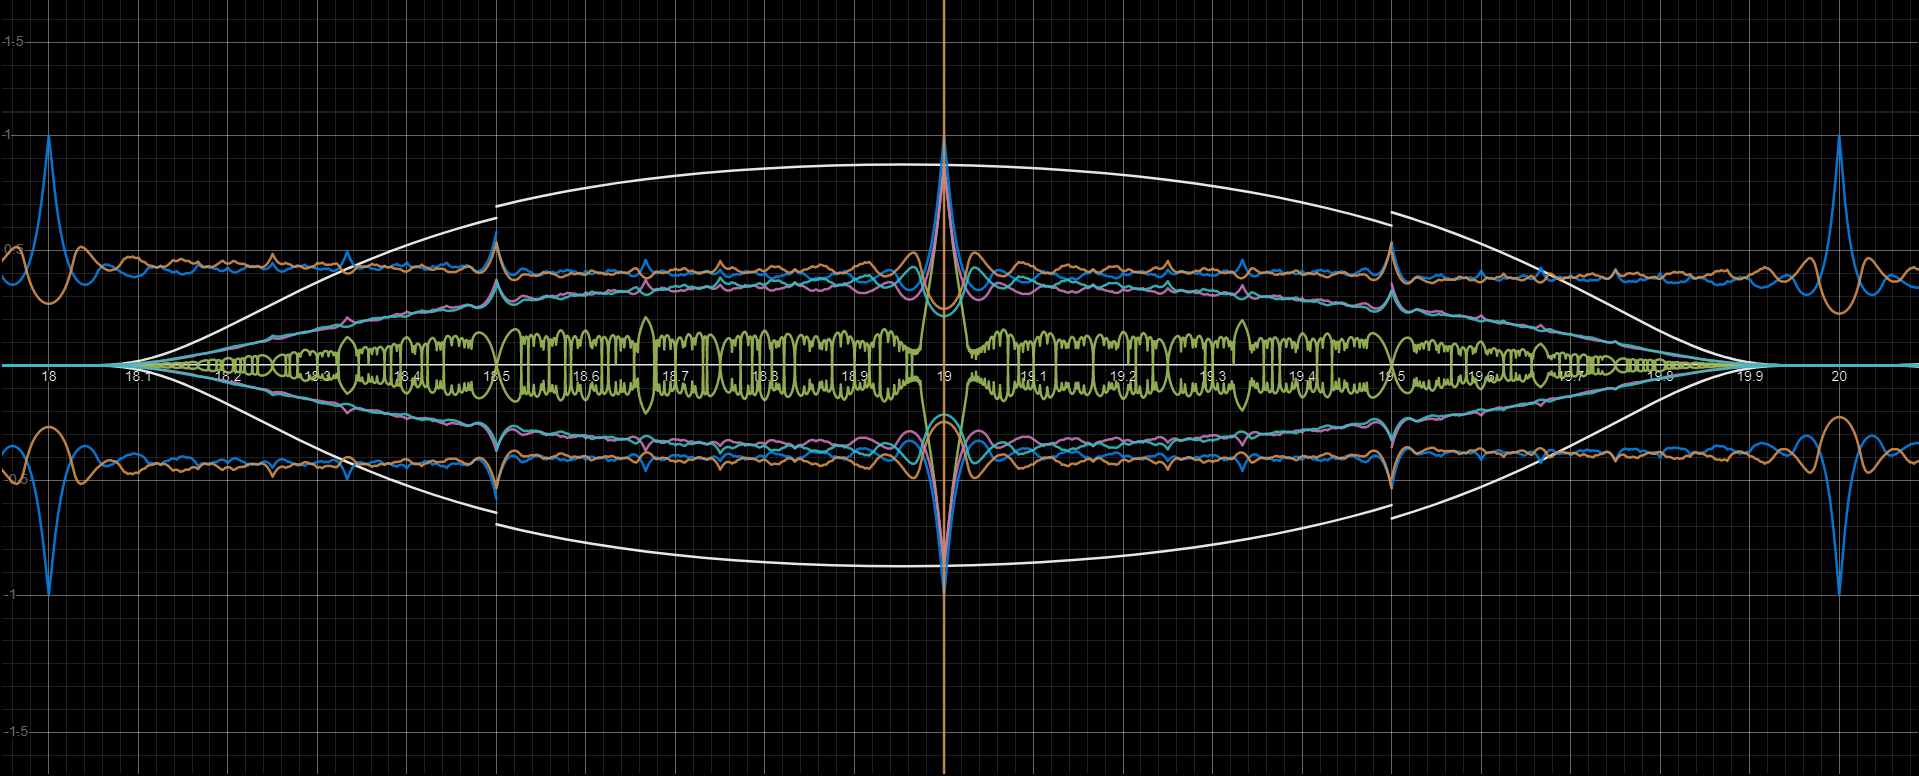
\includegraphics[scale=0.25]{graphs/2D_Real_Graphs/19_waveform_invert}
\end{align*}

\subsection*{j(z), J(z), k(z), K(z), L(z), and B(z) at real(z) = 2 to 14:}
\begin{align*}
\includegraphics[scale=0.30]{graphs/2D_Real_Graphs/sin_cos_tan_primefunc}
\end{align*}

\subsection*{j(z), J(z), k(z), K(z), L(z), and B(z) at real(z) = 6 to 11:}
\begin{align*}
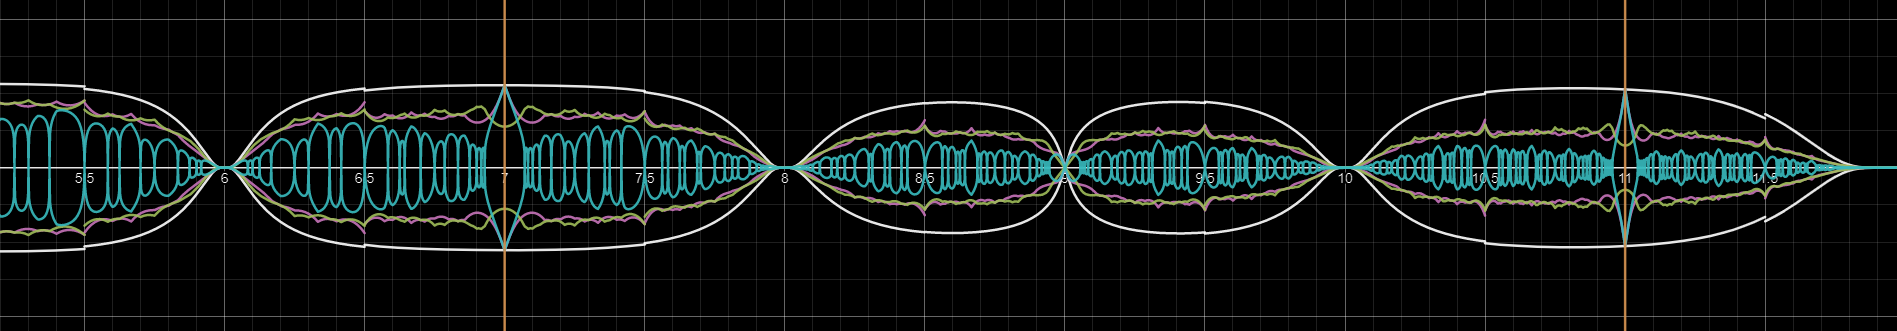
\includegraphics[scale=0.30]{graphs/2D_Real_Graphs/6_11_sin_cos_tan_primefunc}
\end{align*}

\subsection*{j(z), J(z), k(z), K(z), L(z), and B(z) at real(z) = 9:}
\begin{align*}
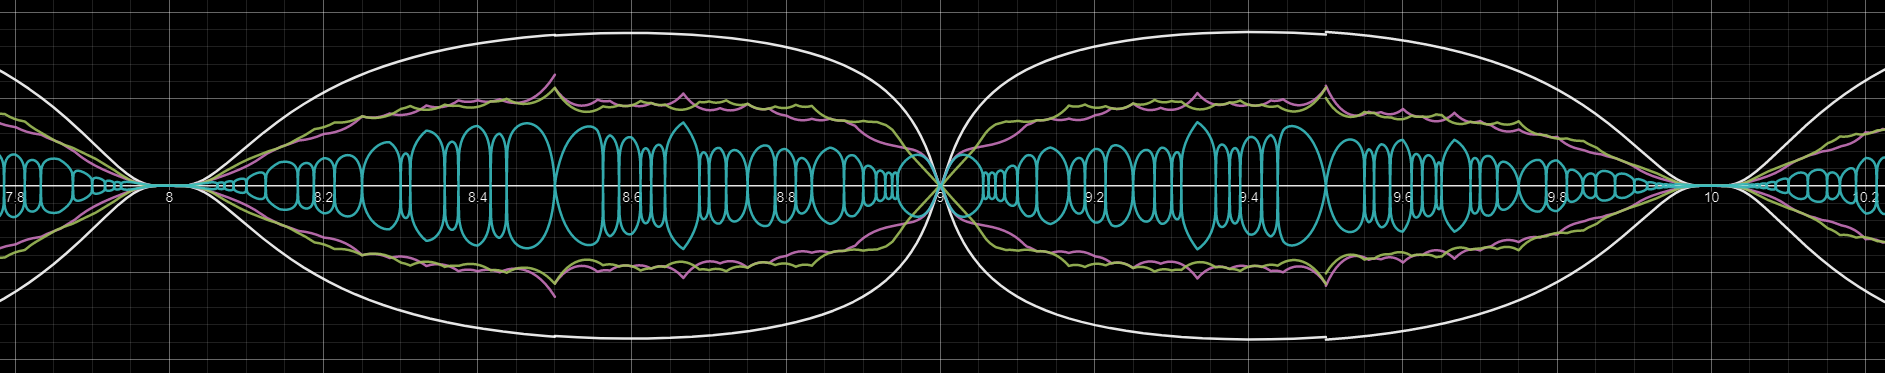
\includegraphics[scale=0.30]{graphs/2D_Real_Graphs/9_sin_cos_tan_primefunc}
\end{align*}

\subsection*{j(z), J(z), k(z), K(z), L(z), and B(z) at real(z) = 11:}
\begin{align*}
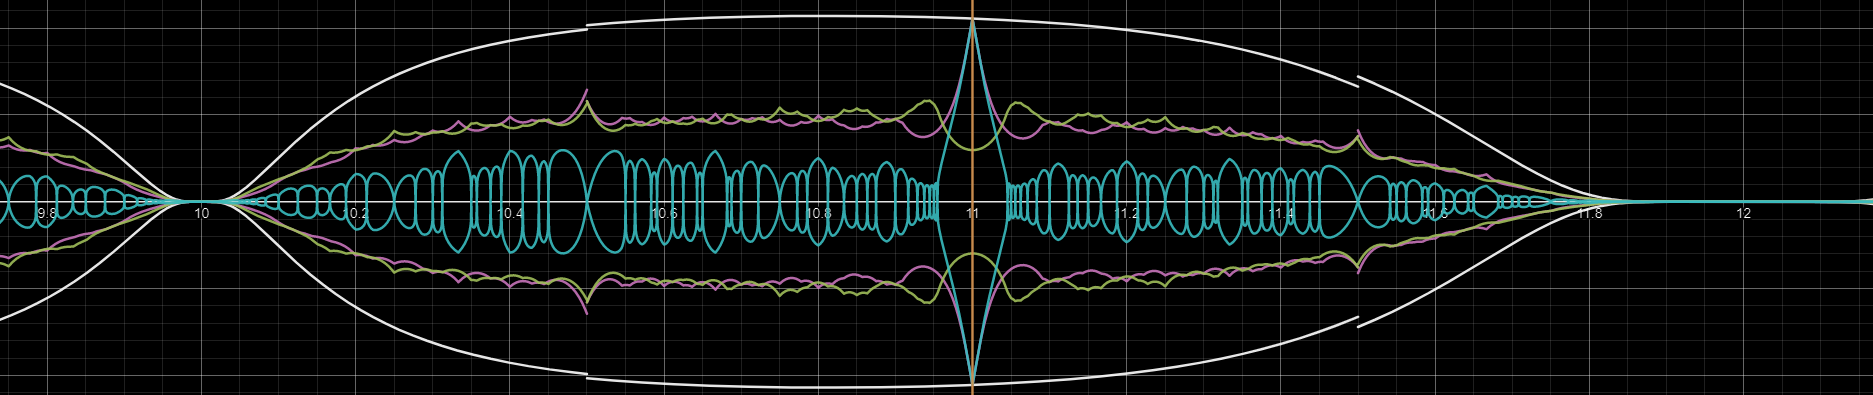
\includegraphics[scale=0.30]{graphs/2D_Real_Graphs/11_sin_cos_tan_primefunc}
\end{align*}

\subsection*{j(z), J(z), k(z), K(z), L(z), and B(z) at real(z) = 13:}
\begin{align*}
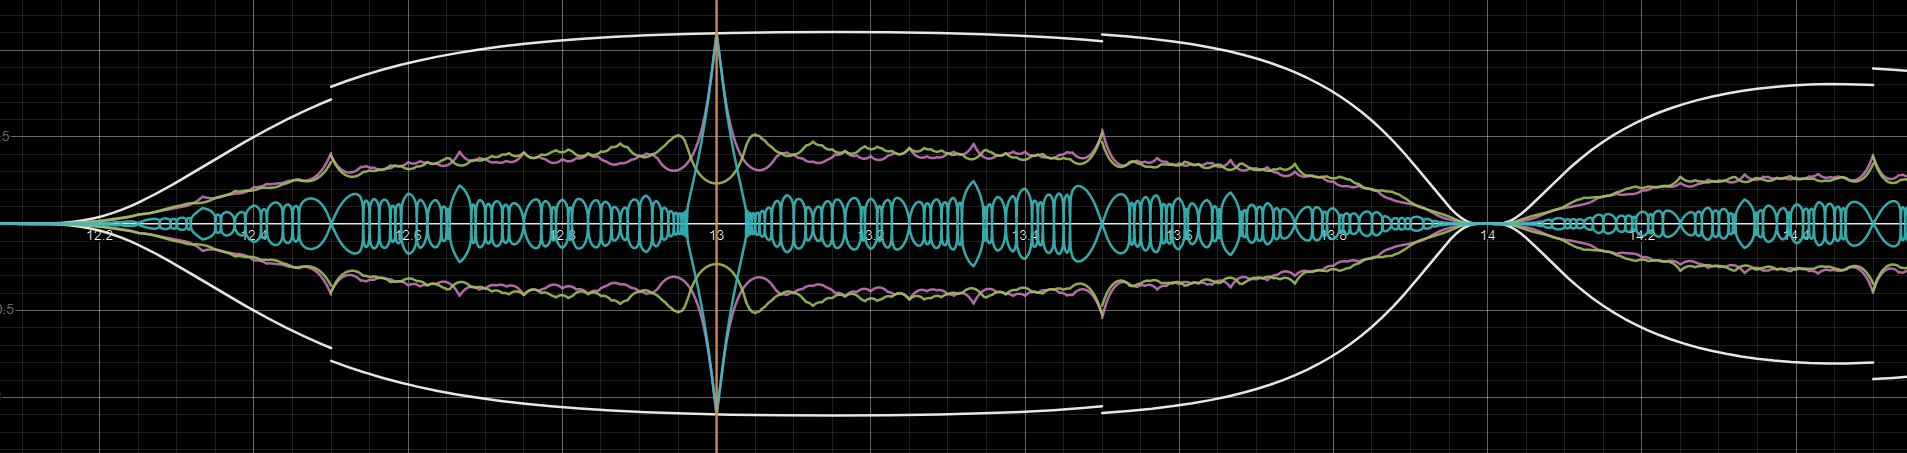
\includegraphics[scale=0.30]{graphs/2D_Real_Graphs/13_sin_cos_tan_primefunc}
\end{align*}

\subsection*{j(z), J(z), k(z), K(z), L(z), and B(z) at real(z) = 15:}
\begin{align*}
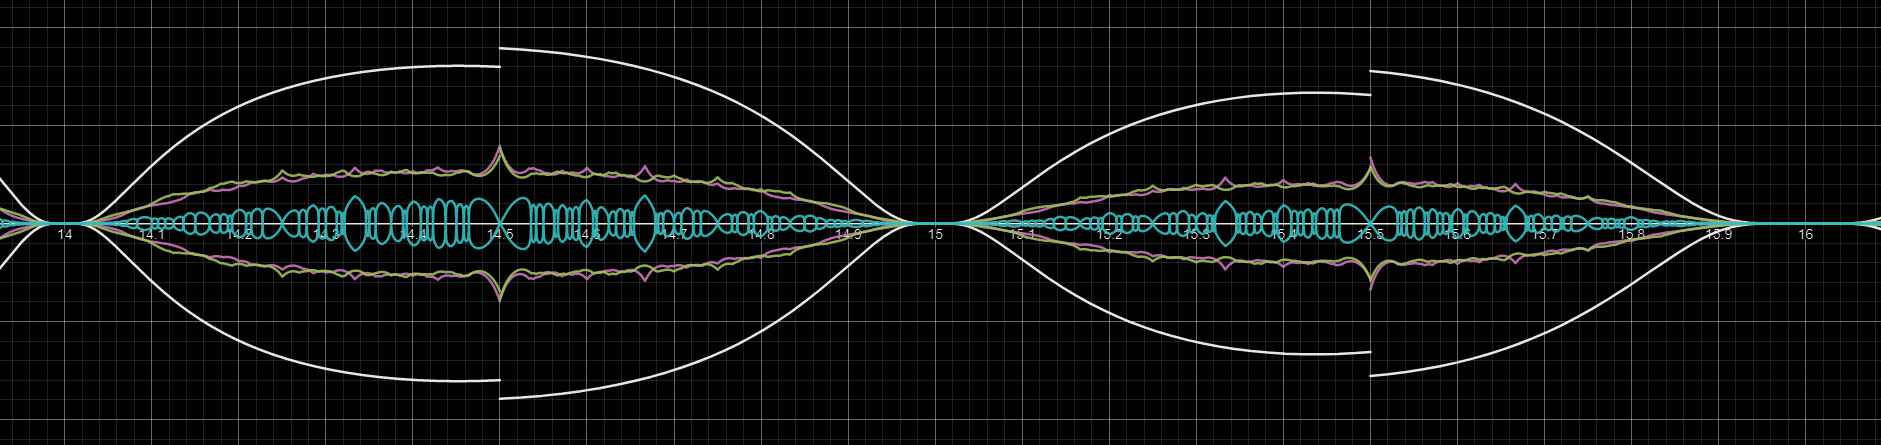
\includegraphics[scale=0.30]{graphs/2D_Real_Graphs/15_sin_cos_tan_primefunc}
\end{align*}

\subsection*{j(z), J(z), k(z), K(z), L(z), and B(z) at real(z) = 17:}
\begin{align*}
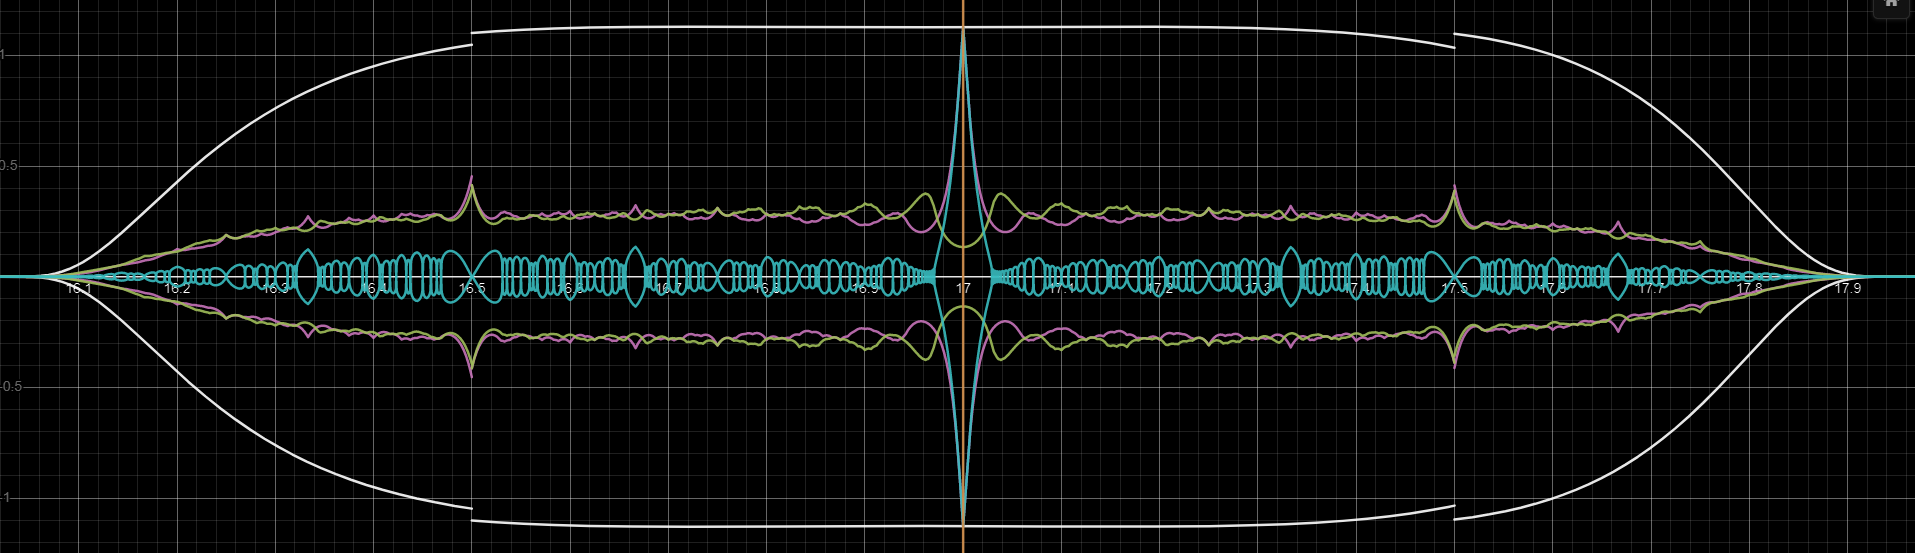
\includegraphics[scale=0.30]{graphs/2D_Real_Graphs/17_sin_cos_tan_primefunc}
\end{align*}

\subsection*{j(z), J(z), k(z), K(z), L(z), and B(z) at real(z) = 19:}
\begin{align*}
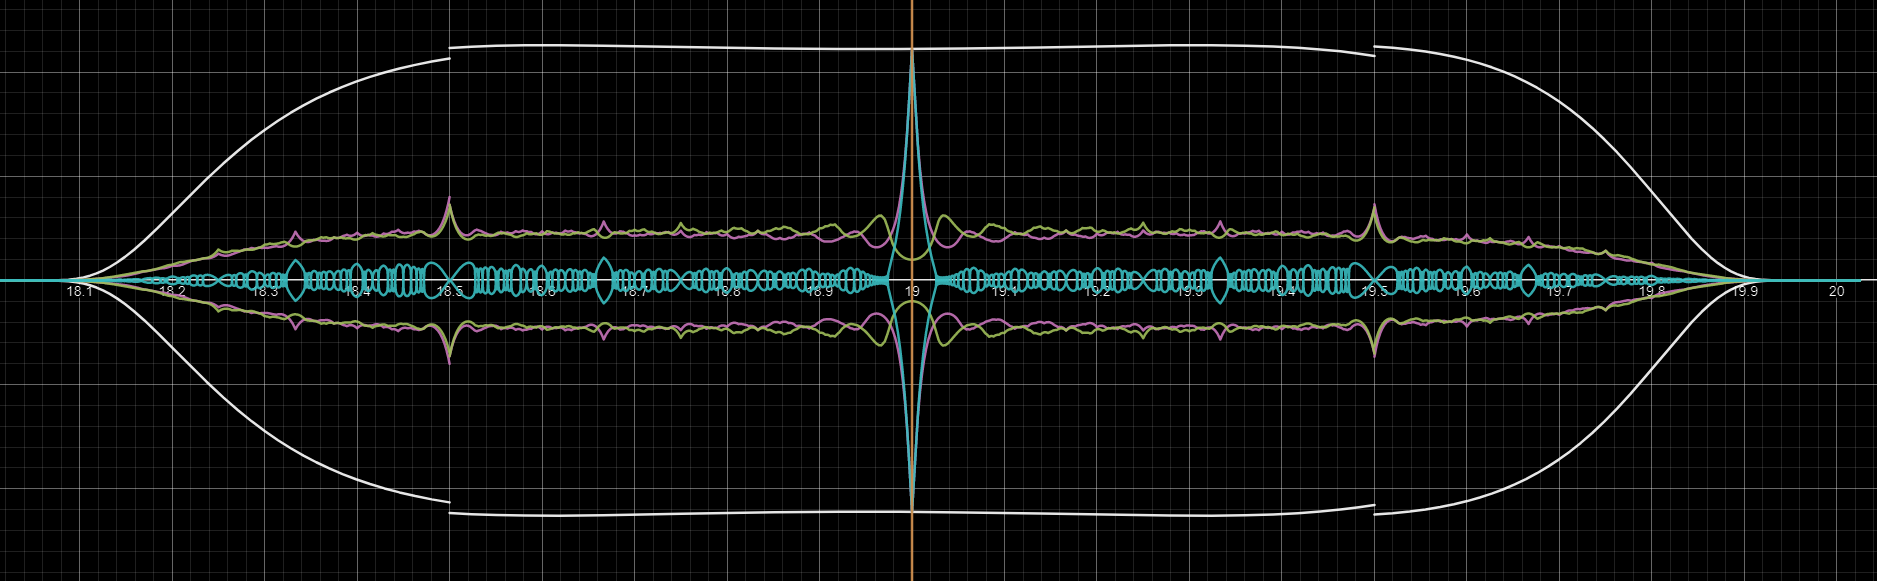
\includegraphics[scale=0.30]{graphs/2D_Real_Graphs/19_sin_cos_tan_primefunc}
\end{align*}

\subsection*{j(z), J(z), k(z), K(z), L(z), and B(z) at real(z) = 21 and 22:}
\begin{align*}
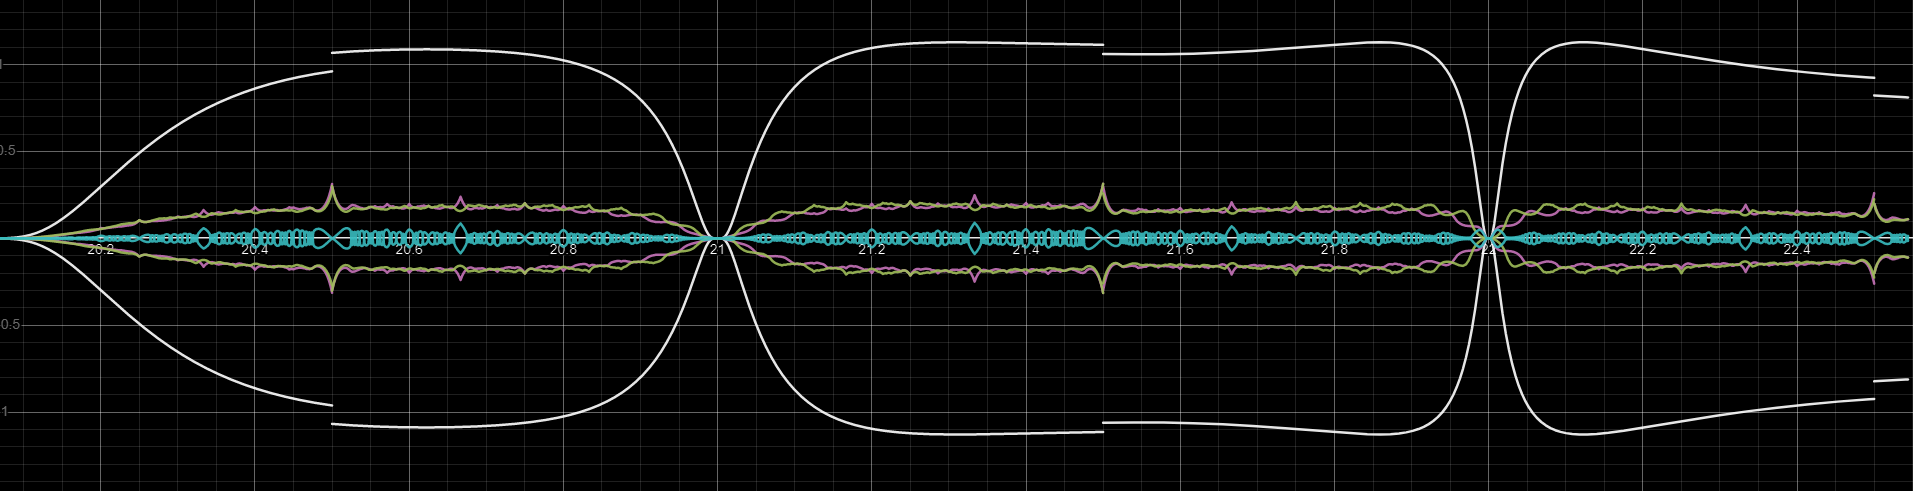
\includegraphics[scale=0.30]{graphs/2D_Real_Graphs/21_22_sin_cos_tan_primefunc}
\end{align*}

\subsection*{j(z), J(z), k(z), K(z), L(z), and B(z) at real(z) = 21 and 22:}
\begin{align*}
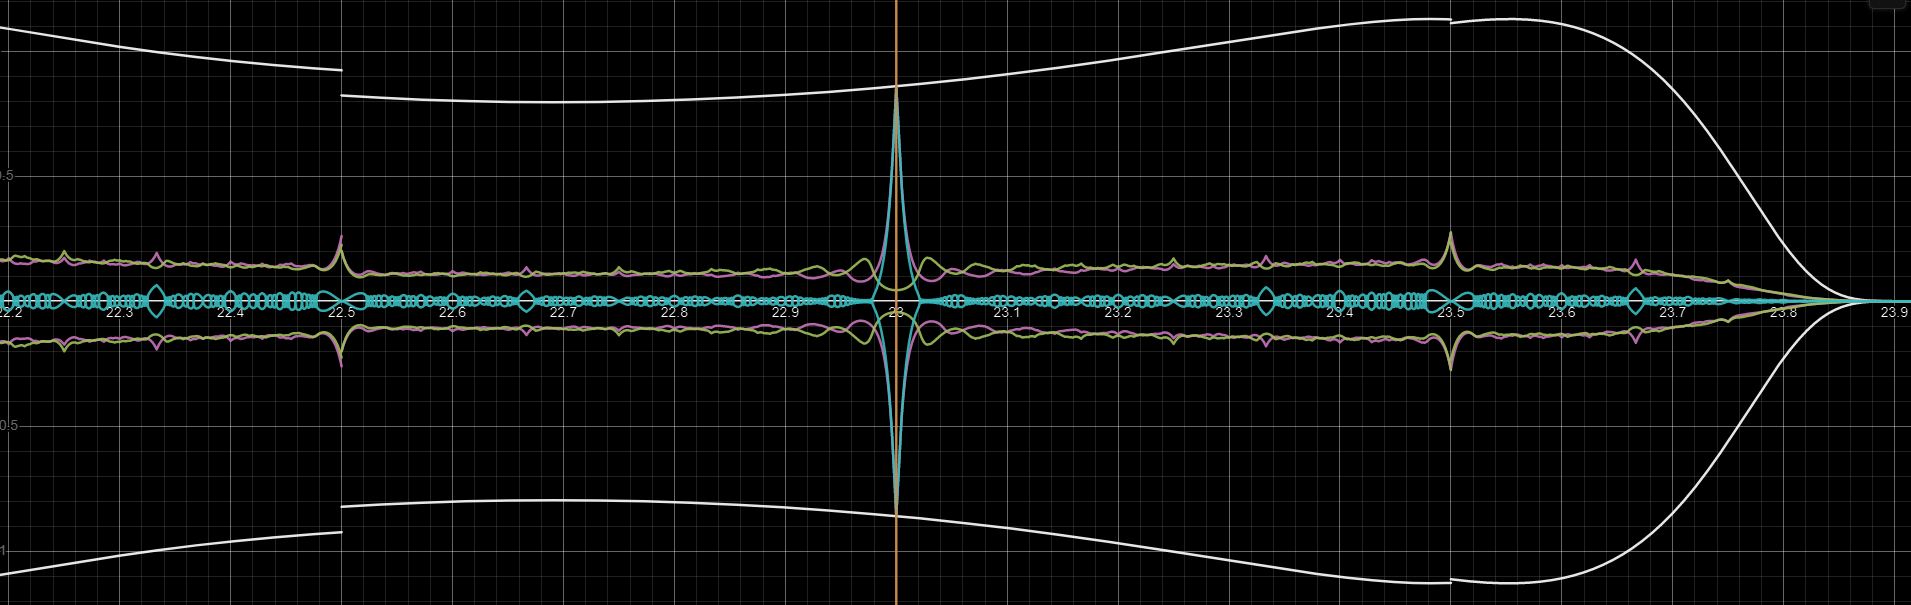
\includegraphics[scale=0.30]{graphs/2D_Real_Graphs/23_sin_cos_tan_primefunc}
\end{align*}

\subsection*{Graph the infinite product representation of zeta at n = 2 to 11 at y = -10, 10 magnification}
\begin{align*}
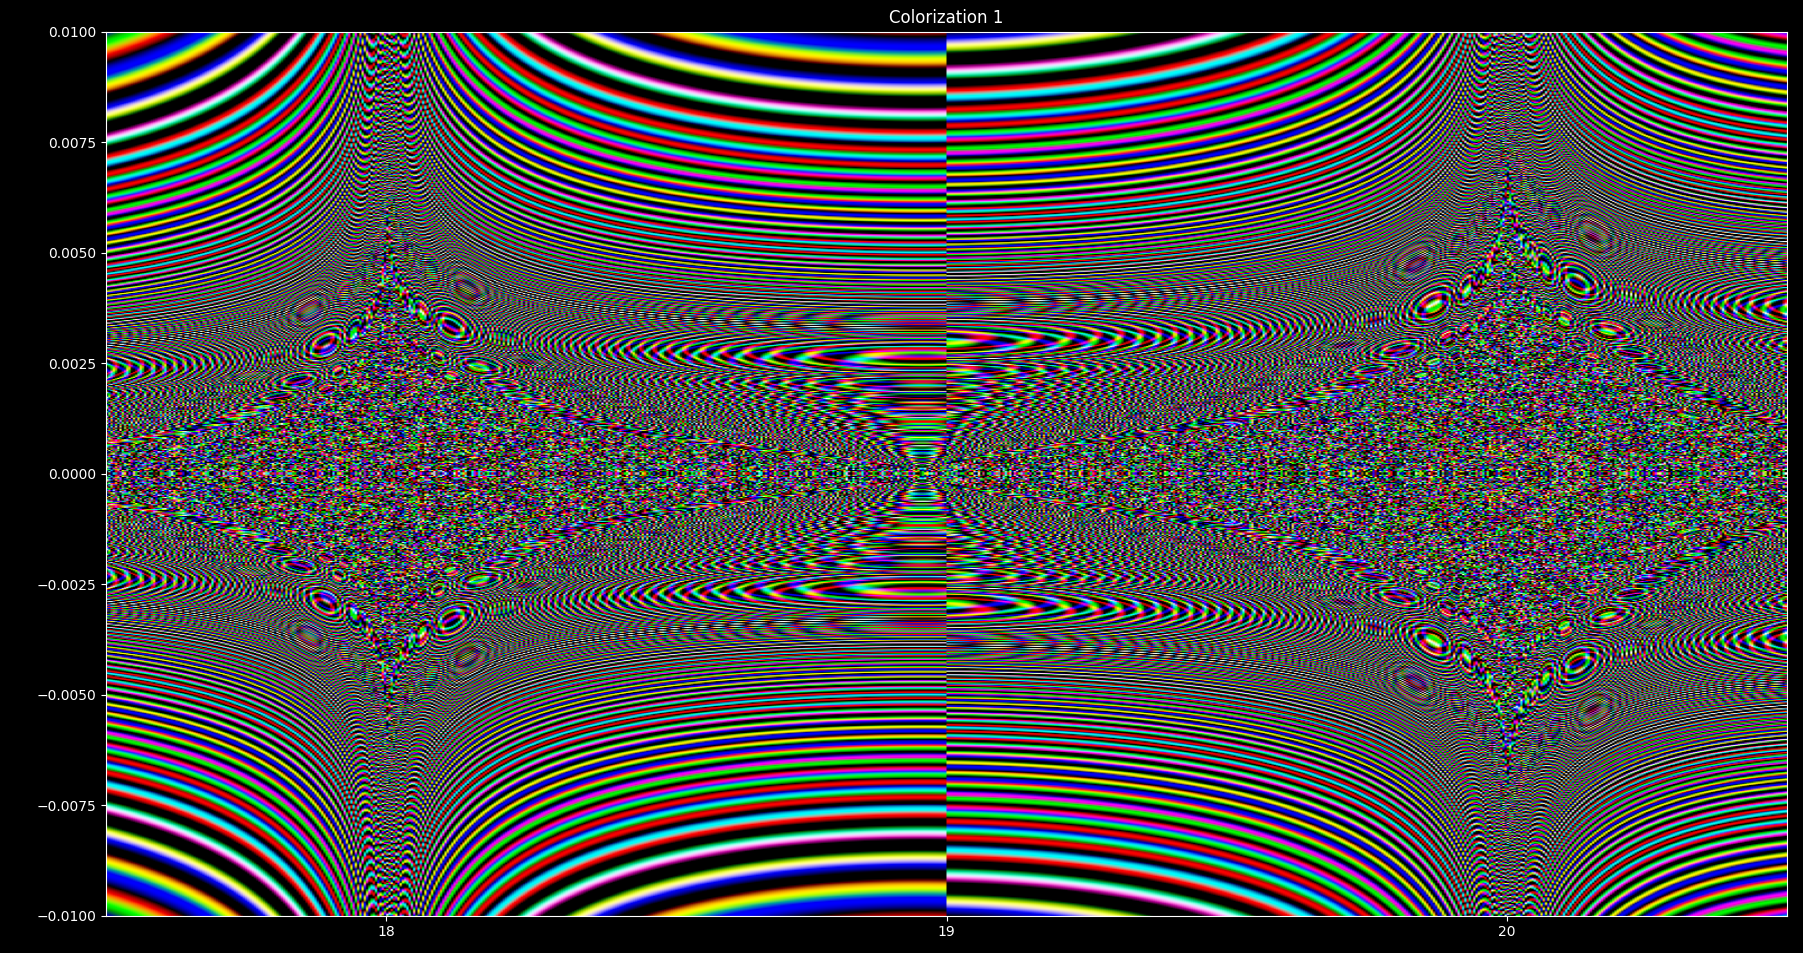
\includegraphics[scale=0.30]{graphs/2D_Complex_Graphs/Reimann_Zeta_function/Complex_product_2_n_2-11_imaginary_component_scalar}
\end{align*}

\subsection*{Graph the infinite product representation of zeta at n = 2 to 11 at y = -100, 100 magnification}
\begin{align*}
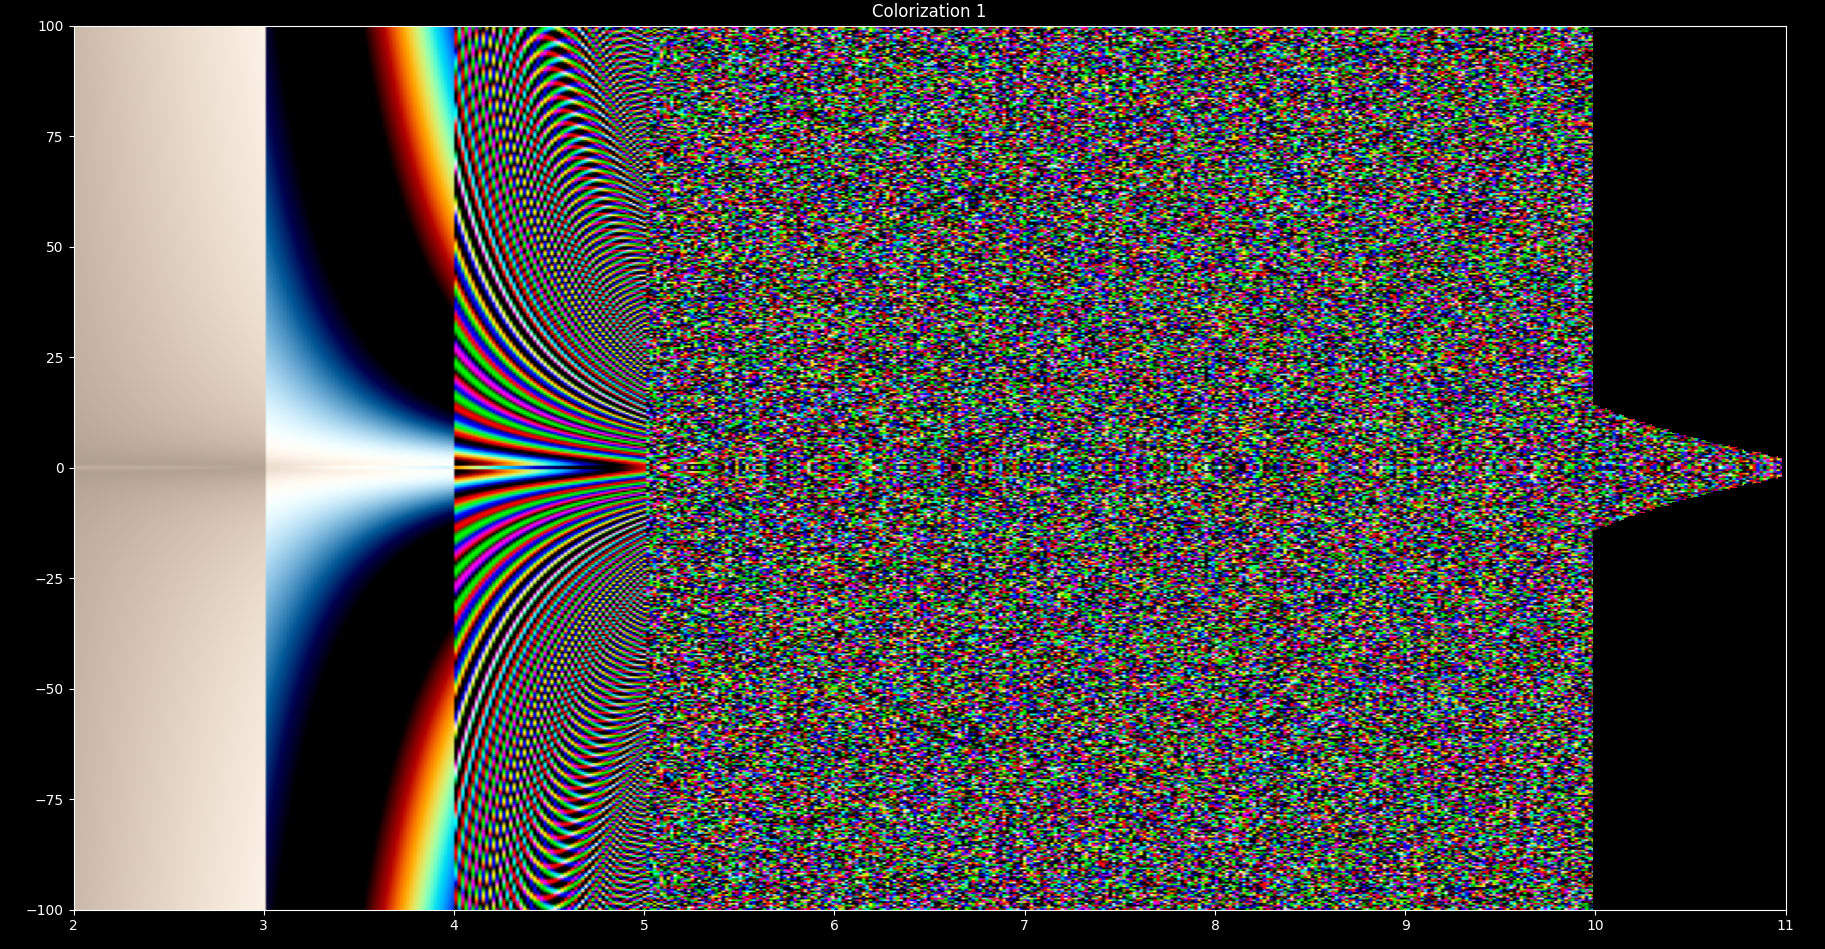
\includegraphics[scale=0.30]{graphs/2D_Complex_Graphs/Reimann_Zeta_function/Complex_product_4_n_2-11_zeta_prod}
\end{align*}

\subsection*{Graph the infinite product b(z) at n = 0 to 84}
\begin{align*}
\includegraphics[scale=0.30]{graphs/2D_Complex_Graphs/Infinite_Product_of_infinite_product_representation_of_sin/Complex_product_11_n0-84_Imaginary_scalar}
\end{align*}

\subsection*{Graph the infinite product b(z) at n = 10 to 28}
\begin{align*}
\includegraphics[scale=0.30]{graphs/2D_Complex_Graphs/Infinite_Product_of_infinite_product_representation_of_sin/Complex_product_12_n10-28_imaginary_scalar}
\end{align*}

\subsection*{Graph the infinite product b(z) at n = 2 to 11 utilizing the imaginary component for magnification}
\begin{align*}
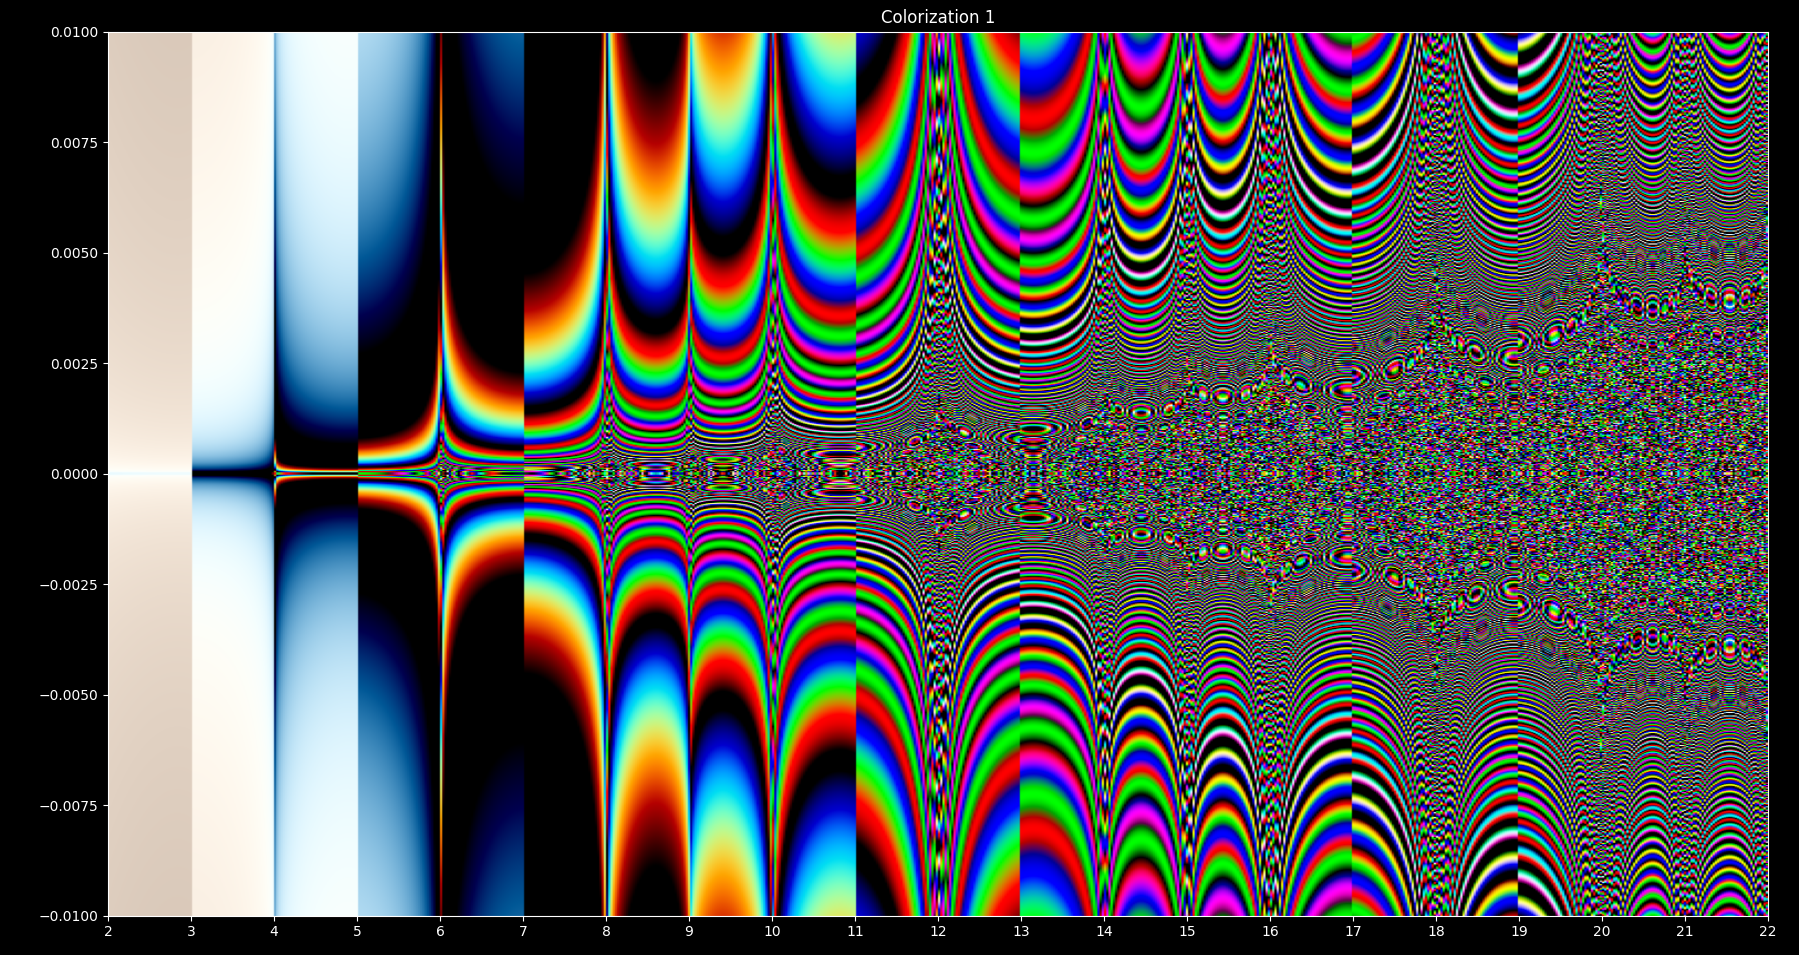
\includegraphics[scale=0.30]{graphs/2D_Complex_Graphs/Infinite_Product_of_infinite_product_representation_of_sin/Complex_product_1_n2-11_imaginary_component_scalar}
\end{align*}


References:

Chan, Erica. "The Sine Product Formula and the Gamma Function." MIT OpenCourseWare, Massachusetts Institute of Technology, 2006, https://ocw.mit.edu/courses/18-104-seminar-in-analysis-applications-to-number-theory-fall-2006/58778de0faae6448c3b0bfb1a1ec4f7a_chan.pdf.

\end{document}